\documentclass[10pt,letterpaper]{phstylee} %,twoside]{phstylee}

\usepackage[utf8]{inputenc}
%\usepackage[T1]{fontenc}
\usepackage[dvips,final]{epsfig}
\usepackage[spanish]{babel}
\usepackage{amsthm}
\usepackage{amsmath}
\usepackage{amssymb}
\usepackage{cite}
\usepackage{amsfonts}
\usepackage{amsxtra}
%\usepackage{varioref}
%\usepackage{multicol}
%\usepackage{float}
%\usepackage{rotate}
\usepackage{color}
%\usepackage{enumerate}
%\usepackage{pmat}
\usepackage{graphicx}
%\usepackage{hangcaption}
%\usepackage{latexsym}
%\usepackage{dsfont}

\allowdisplaybreaks

%%%%%%%%%%%%%%%%%%%%%
%      DIRECTORIO DONDE BUSCA LAS FIGURAS

\graphicspath{{figuras/}}

% hyper references packages, it should be the LAST
%\usepackage{citesort}
%\usepackage[bookmarks=true,bookmarksnumbered,colorlinks=true,linkcolor=black,citecolor=black,pdfstartview=FitH,linktocpage,dvipdfm]{hyperref}
%\usepackage[dvips]{hyperref}
%\hypersetup{
%  colorlinks=true, %true,
%  linkcolor=black,
%  citecolor=black,
%  linktocpage=true,
%  pdftitle={Estimaci\'on de estado en sistemas observados a trav\'es de canales con p\'erdida de datos.},
%  pdfauthor={Miguel Sol\'is.}
%} 


\addtolength{\topmargin}{-30pt}
\linespread{1.1} %tama\~no de la l\'inea
\makeindex
\spanishdecimal{.}

%%%%%%%%%%%%%%%%%%%%%%%%%%%%%%%%%%%%%%%%%%%%%%%%%%%%%%%%%%%%
%%%%%%%%%%%%%%%%%%%%%%%%%%%%%%%%%%%%%%%%%%%%%%%%%%%%%%%%%%%%
\begin{document}
%\layout
%--------------------PORTADA--------------------------------
%
\setcounter{tocdepth}{2}
\input portada.tex
\cleardoublepage

%--------------------RESUMEN--------------------------------

\pagestyle{fancyplain}

%\cleardoublepage
%\newpage
%\thispagestyle{empty}
%\mbox{}
%\cleardoublepage

\pagenumbering{roman}

\chapter*{Agradecimientos}
Gracias a todos los involucrados en este trabajo, ya sea de forma directa o indirecta.

Gracias a mi familia y amigos.

%\input agradecimientos.tex

\cleardoublepage
\newpage
\thispagestyle{empty}
\mbox{}
\cleardoublepage

\chapter*{Resumen}
\input resumen.tex

%\cleardoublepage
\newpage
%\thispagestyle{empty}
%\mbox{}
%\cleardoublepage

\chapter*{Abstract}
\input abstract.tex

\cleardoublepage
\newpage
\thispagestyle{empty}
\mbox{}
\cleardoublepage
 
%--------------------\'iNDICE---------------------------------
\cleardoublepage
%\pagenumbering{arabic}
\chapter*{Glosario}
\input glosario.tex
\mbox{}
\cleardoublepage

\tableofcontents
%-------------------CAP\'iTULOS-------------------------------
%%%%%%%%%%%%%%%%%%%%%%%%%%%%%%%%%%%%%%%%%%%%%%%%%%%%%%%%%%%%
%
\cleardoublepage
\pagenumbering{arabic}
\chapter{Introducci\'on}
\label{cap:introduccion}
\chapter{INTRODUCCI�N Y OBJETIVOS}

El proyecto``\(\tau\)-HyperNEAT: Retardos de Tiempo en una Red HyperNEAT para Aprendizaje de Caminatas en Robots con Extremidades M�viles'' pretende incorporar conceptos temporales en una red neuronal HyperNEAT incluyendo retardos de tiempo adicionales a los pesos en las conexiones entre neuronas, permitiendo as� generar caminatas en robots con distinta cantidad de grados de libertad (ver Figura \ref{fig:robots}), a trav�s de simulaciones en entornos virtuales, de forma m�s �ptima y obteniendo resultados m�s cercanos a comportamientos encontrados en la naturaleza.

\begin{figure}[ht!]
	\centering
	\begin{subfigure}[b]{0.45\textwidth}
		\centering
        \includegraphics[width=\textwidth]{fig/QUADRATOT.png}
        \caption{Quadratot}
        \label{fig:quadratot}
    \end{subfigure}
    ~
	\begin{subfigure}[b]{0.45\textwidth}
		\centering
        \includegraphics[width=\textwidth]{fig/ARGOV2.png}
        \caption{ArgoV2}
        \label{fig:argov2}
    \end{subfigure}
    \caption{\textbf{Robots con distinto n�mero de grados de libertad y diferentes geometr�as. } En la figura se aprecia dos robots, Quadratot y ArgoV2, ambos de 4 extremidades, y de 9 y 12 grados de libertad totales respectivamente.}
    \label{fig:robots}
\end{figure}

\section{OBJETIVOS DEL PROYECTO}

\begin{description}
\item[\textbf{Objetivo 1}] Proponer un red neuronal usando HyperNEAT que incluya retardos de tiempo en sus conexiones.

\item [\textbf{Objetivo 2}] Desarrollar el software necesario para manejar el entorno de simulaci�n a usar en el trascurso del proyecto.

\item [\textbf{Objetivo 3}] Usar la nueva red neuronal en tareas de aprendizaje de caminatas en robots con extremidades m�viles.
\end{description}

\section{TRABAJOS A DESARROLLAR Y RESULTADOS ESPERADOS}

El proyecto se inicia en base a estudios e implementaciones previas de redes NEAT\footnote{\url{https://github.com/osilvam/NEAT}} y HyperNEAT\footnote{\url{https://github.com/osilvam/HyperNeat}} para la generaci�n de caminatas en robots con extremidades m�viles en entornos virtuales de simulaci�n\footnote{como parte de un trabajo de investigaci�n realizado por los alumnos de Ingenier�a Civil Electr�nica Pascal Sigel Olivares y Oscar Silva Mu�oz encabezados por la profesora del Departamento de Electr�nica de la Universidad T�cnica Federico Santa Mar�a Dr. Mar�a Jos� Escobar Silva.}, con los cuales se obtuvieron resultados exitosos. A partir de esto es que se plantea la incorporaci�n de retardos de tiempo a una red HyperNEAT de forma de implementar computacionalmente la nueva red neuronal propuesta llamada \(\tau\)-HyperNEAT. Luego se debe comparar el desempe�o de \(\tau\)-HyperNEAT versus el desempe�o de su predecesor entrenando caminatas en los robots, el cual se espera que sea mejor. La correcta generaci�n y evoluci�n de caminatas en un entrenamiento est� sujeta a una funci�n de desempe�o en base a las variables observadas en el robot, por lo que se debe realizar un estudio exhaustivo de cu�l es la funci�n de desempe�o que mejor describe a una correcta caminata. Para el desarrollo de los entrenamientos de caminatas en los robots en entornos virtuales es necesario implementar un modelo para cada robot, con el fin de observar las caminatas generadas y emular correctamente las din�micas que se presentar�an en un entorno real \footnote{Como trabajo futuro de esta memoria se propone lograr traspasar de manera posterior los resultados obtenidos a los robots reales.}. Adem�s, se debe desarrollar el software necesario para la comunicaci�n entre el programa de entrenamiento y el programa que provee el entorno virtual de simulaci�n (el cual soporta comunicaci�n por sockets).

La comparaci�n de los resultados de las caminatas obtenidos entre HyperNEAT y \(\tau\)-HyperNEAT debe realizarse observando tanto el aspecto visual final de las caminatas obtenidas, como adem�s la evoluci�n de dichas caminatas a lo largo del proceso de entrenamiento, medida a trav�s de la funci�n de desempe�o antes mencionada, la cual eval�a cuantitativamente las caminatas generadas. Luego se debe comparar cuan influyentes fueron los retardos de tiempo incluidos en la red HyperNEAT observando la estructura y conexiones de la red \(\tau\)-HyperNEAT finalmente obtenida para obtener las conclusiones del trabajo propuesto.

Al culminar el Proyecto ``\(\tau\)-HyperNEAT: Retardos de Tiempo en una Red HyperNEAT para Aprendizaje de Caminatas en Robots con Extremidades M�viles'', se espera poder obtener caminatas naturales y arm�nicas en robots con extremidades m�viles de manera m�s �ptima a las obtenidas solo con una red HyperNEAT. De manera m�s general se pretende obtener una red neuronal m�s robusta y eficiente que permita resolver problemas reales con dependencias temporales. Adem�s se espera generar un software robusto que permita una correcta comunicaci�n con el entorno de simulaci�n a usar para proveer esta herramienta a proyectos futuros en donde se requiera emular sistemas reales complejos.

Adem�s del problema mismo de la generaci�n de caminatas en robots con extremidades m�viles, se encuentra la tarea de simular virtualmente el modelo de cada robot, ya que la mayor�a de las veces realizar pruebas en plataformas reales es inalcanzable, por elevados costos de adquisici�n de los equipos; muy poco pr�ctico ya que requiere de una constante y prolongada intervenci�n de personas; o muy peligroso, ya que cualquier problema o error podr�a incurrir en el deterioro del equipo o inclusive podr�a atentar contra la seguridad de las mismas personas que realizan los experimentos. Es por esto que esta memoria contempla la implementaci�n de una herramienta de software que permita al usuario trabajar con modelos virtuales simulados de forma f�cil y r�pida.

Para el trabajo de simulaci�n en el �rea de la rob�tica existen variadas opciones con distintos niveles de dificultad y costo de uso dependiendo del p�blico objetivo para el cual est� pensado. Es por esto que para el desarrollo de esta memoria se propone el uso de una herramienta de f�cil acceso, tanto por el nivel de conocimiento que requiere su uso como su accesibilidad de descarga y sencillo manejo, con el objetivo de que el software a realizar este al alcance de uso de cualquier persona. Esto busca acercar a las personas a trabajar en el �rea de la rob�tica incit�ndolas con herramientas de f�cil acceso y manejo.



%
%%%%%%%%%%%%%%%%%%%%%%%%%%%%%%%%%%%%%%%%%%%%%%%%%%%%%%%%%%%%%
%
\cleardoublepage
\chapter{Estado del arte de m\'etodos evolutivos para la caminata de robots}
\label{cap:estado_del_arte}
En el �rea de redes neuronales que hacen uso de neuroevoluci�n y algoritmos gen�ticos se puede observar el trabajo realizado por el investigador Kenneth O. Stanley, siendo el primer art�culo de inter�s el que relata el desarrollo de NEAT \cite{neat}, Neuroevoluci�n a trav�s del Aumento de Topolog�as, el cual supera en pruebas comparativas a redes con topolog�as fijas en tareas de aprendizaje reforzado. Stanley asume que el aumento en la eficiencia se debe al uso de un m�todo de cruce entre diferentes topolog�as, a la clasificaci�n por especies de redes diferenciadas por su topolog�a y cambios en ella, y el crecimiento incremental a partir de una estructura m�nima.

Una continuaci�n del desarrollo de NEAT es HyperNEAT \cite{hyperneat}, Hipercubo basado en Neuroevoluci�n a trav�s del Aumento de Topolog�as, igualmente desarrollado por Stanley, el cual emplea una codificaci�n indirecta llamada conectivo Compositional Pattern Producing Network (conectivo CPPNs), que puede producir un patr�n de conectividad con simetr�as y esquemas repetidos interpretado por el patr�n espacial generado dentro de un hipercubo. La ventaja de este enfoque es que es posible explotar la geometr�a de la tarea mediante el mapeo de sus regularidades en la topolog�a de la red, desplazando con ello la dificultad del problema lejos de la dimensionalidad de este hacia la estructura misma del problema.

En el �rea de generaci�n de caminatas en robots con extremidades m�viles existe una vasta cantidad de investigaciones relacionadas tanto con el uso de HyperNEAT, algoritmos gen�ticos en general u otro tipo de t�cnicas que se expondr�n a continuaci�n.

Investigadores de la Universidad de Cornell el a�o 2004 publicaron ``Evolving Dynamic Gaits on a Physical Robot'' \cite{zykov}, en donde formularon un algoritmo gen�tico para entrenar un controlador de lazo abierto para la generaci�n de una caminata en un robot conformado por dos plataformas Stewart, evolucionando en b�squeda de optimizar su velocidad y su patr�n de movimiento garantizando al mismo tiempo el ritmo de estos.

Otros investigadores del Centro de Investigaci�n Ames, de la NASA, el a�o 2005 publicaron ``Autonomous Evolution of Dynamic Gaits with Two Quadruped Robot'' \cite{hornby}, en donde relatan c�mo han desarrollado un algoritmo de evoluci�n para generar caminatas din�micas en dos robos cuadr�pedos, OPEN-R y ERS-110 de la marca Sony, midiendo el desempe�o de las caminatas con los distintos sensores incorporados en ellos.

En el 2009, el investigador Jeff Clune junto a otros publicaron ``Evolving Coordinated Quadruped Gaits with the HyperNEAT Generative Encoding'' \cite{clune}, en donde demuestra c�mo es posible desarrollar caminatas en robos cuadr�pedos sin realizar un trabajo manual para resolver el problema usando HyperNEAT.

En el 2011, investigadores de la Universidad de Cornell junto a un investigador de la Universidad de Chile publicaron ``Evolving Robot Gaits in Hardware: the HyperNEAT Generative Encoding Vs. Parameter Optimization'' \cite{yosinski}, en donde presentan la investigaci�n de variados algoritmos para la generaci�n autom�tica de caminatas sobre un robot cuadr�pedo, en donde se comparan dos clases, los de b�squeda local de modelos de movimientos parametrizados y la evoluci�n de redes neuronales artificiales usando HyperNEAT. Aqu� concluyeron que las caminatas desarrolladas con HyperNEAT fueron considerablemente mejores a las desarrolladas con los otros m�todos de b�squeda local parametrizada, y produjo caminatas casi nueve veces m�s r�pidas que caminatas generadas a mano.

En el a�o 2013, un grupo de investigadores de la Universidad de Cornell, Universidad de Oslo y Universidad de Wyoming publicaron en conjunto ``Evolving Gaits for Physical Robots with the HyperNEAT Generative Encoding: The Benefits of Simulation'' \cite{lee}, en el cual plantean y confirman la hip�tesis de que los resultados de las caminatas generadas con HyperNEAT en un entorno simulado superan con creces a las generadas en un entorno real.

Recientemente investigadores de la Universidad de la Coru�a han propuesto una extensi�n del algoritmo NEAT propuesto por Stanley llamado \(\tau\)-NEAT \cite{caamano} debido a que NEAT no es siempre fiable cuando existen manejos de variables temporales dentro de la tarea a solucionar debido a la falta de elementos temporales expl�citos dentro de la topolog�a de la red NEAT. Es por esta raz�n que el algoritmo \(\tau\)-NEAT propuesto incluye la posibilidad de incluir retardos variables en las conexiones de la red NEAT, afectando tanto a las conexiones directas como recurrentes de la red.

El software de simulaci�n que se usar� para el desarrollo de esta memoria se llama V-REP \cite{vrep}, Virtual Robot Experimentation Plataform, desarrollado por Coppelia Robotics GmbH en Zurich, Suiza, el cual posee versiones tanto pagas como gratuitas. La versi�n educacional de este software es completamente gratuita y posee todas las funcionalidades del programa completo. Este software posee una API desarrollada en una gran variedad de lenguajes de programaci�n, permitiendo as� manejar todos los aspectos del programa y la simulaci�n desde el exterior a trav�s de sockets. Esta API ser� usada por la herramienta de software a desarrollar para el trabajo con los experimentos tanto en el entorno virtual como en el real.

Con respecto a la herramienta de software que se implementar� para manejar transparentemente las plataformas rob�ticas en el entorno de simulaci�n y entorno real no se conoce implementaci�n alguna disponible, por lo que se cree ser� una gran contribuci�n a trabajos futuros.
%
%%%%%%%%%%%%%%%%%%%%%%%%%%%%%%%%%%%%%%%%%%%%%%%%%%%%%%%%%%%%%%
%
\cleardoublepage
\chapter{Base Te\'orica}
\label{cap:base_teorica}
\chapter{BASE TE�RICA}

En este cap�tulo se presentar� una introducci�n te�rica de la herramienta de neuroevoluci�n HyperNEAT y sus componentes, necesaria para la implementaci�n de \(\tau\)-HyperNEAT.

\section{COMPOSITIONAL PATTERN PRODUCING NETWORKS}

La representaci�n es uno de los elementos principales en la IA. Particularmente cuando un problema involucra b�squedas, una buena representaci�n del espacio de soluci�n puede hacer la diferencia entre �xito y fracaso. En computaci�n evolutiva, como los genomas tradicionales de tama�o fijo y codificaciones directas alcanzan sus l�mites, la importancia de la representaci�n se ha movido al frente de la investigaci�n. %Mientras tanto, la biolog�a sigue siendo una constante motivaci�n que nos recuerda que tan lejos es posible llegar. 

En biolog�a, los genes en el ADN representan estructuras tremendamente complejas con miles de millones de partes interconectadas, tal como lo es el cerebro humano. Sin embargo el ADN no contiene miles de millones de genes, de echo, solo treinta mil genes codifican todo el cuerpo. Esta es la raz�n para creer que el descubrimiento de sistemas tan complejos como el de los seres humanos es solo posible a trav�s de una extraordinariamente eficiente codificaci�n, como se ve en la naturaleza. Un proceso clave en la codificaci�n en la naturaleza es la reutilizaci�n de genes ya que el mismo gen puede ser activado en cualquier lugar y en cualquier momento en el proceso de desarrollo. As� un peque�o conjunto de genes puede codificar un conjunto mucho mas grande de componentes estructurales.

Esta observaci�n ha inspirado un campo activo de investigaci�n en la \textsl{codificacion de desarrollo} artificial. El objetivo es encontrar la correcta abstracci�n del desarrollo natural, por un computador corriendo un algoritmo evolutivo, de modo que pueda comenzar a descubrir la complejidad en una escala natural. Una faceta com�n de algunas abstracciones es que un estado de un componente individual del fenotipo en un momento del desarrollo afecta los estados de los componentes de la misma vecindad en el futuro, es decir, el desarrollo se despliega a trav�s de interacciones locales. Debido a que ninguna abstracci�n se ha acercado hasta ahora a descubrir el nivel de complejidad visto en la naturaleza, sigue siendo de gran inter�s identificar las propiedades de abstracci�n que dan lugar a una codificaci�n eficiente.

El principal aporte detr�s de ``Compositional Pattern Producing Networks'' (CPPNs), es que es posible describir directamente las relaciones estructurales que resultan de un proceso de desarrollo sin simular el proceso mismo. En su lugar, la descripci�n es codificada a trav�s de una composici�n de funciones, cada una de estas basadas en el patr�n de gradientes observado en embriones en la naturaleza.

Desde una perspectiva estructura CPPNs y ANNs son muy similares debido a que m�todos designados para evolucionar ANNs tambi�n pueden evolucionar CPPNs. En particular, el m�todo de ``NeuroEvolution of Augmenting Topologies'' (NEAT) es una buena opci�n para evolucionar CPPNs porque NEAT incrementa la complejidad de las redes a medida que evolucionan generaci�n tras generaci�n, permitiendo que se generen cada vez regularidades mas elaboradas.

En el siguiente secci�n se introducir�n importantes caracter�sticas de patrones de desarrollo.

\subsection{PATRONES DE DESARROLLO}

El desarrollo produce patrones y la evoluci�n produce secuencias de patrones generaci�n tras generaci�n. Los patrones incluyen regularidades y las regularidades son las que hacen posible una reutilizaci�n en la codificaci�n. Sin regularidad, la misma informaci�n no puede producir distintas partes de un mismo fenotipo, reduciendo mucho las ventajas del desarrollo. A continuaci�n se mencionaran caracter�sticas generales de patrones observados en organismos de la naturaleza que tambi�n puede buscarse en fenotipos evolucionado artificialmente.

\begin{itemize}
\item[\textbf{Repetici�n }] M�ltiples instancias de la misma subestructura es un sello distintivo de los organismos biol�gicos. Desde las c�lulas de todo el cuerpo hasta las neuronas del cerebro, las mismas estructuras se repiten una y otra vez en un �nico organismo. La repetici�n en el fenotipo tambi�n se llama auto similitud.
\item[\textbf{Repetici�n con variaciones }] Frecuentemente estructuras se encuentran repetidas pero no de forma completamente id�nticas. Esto se ve de forma frecuente en toda la naturaleza, como por ejemplo en las vertebras de una columna o en los mismos dedos de una mano, cada una de sus componentes posee la misma estructura pero con distintas variaciones.
\item[\textbf{Simetr�a }] A menudo las repeticiones ocurren a trav�s de las simetr�as, como cuando los lados derecho e izquierdo del cuerpo son id�nticas, produci�ndose una simetr�a bilateral.
\item[\textbf{Simetr�a imperfecta }] Mientras que un tema sim�trico general es observable en muchas estructuras biol�gicas, muchas veces no son perfectamente sim�tricas. Tal simetr�a imperfecta es una caracter�stica com�n de repetici�n con variaciones. El cuerpo humano es sim�trico en general, pero no es equitativo en ambos lados; algunos �rganos solo aparecen en uno de los lados, y un lado es generalmente dominante sobre el otro.
\item[\textbf{Regularidades elaboradas }] Durante muchas generaciones, regularidades son a menudo elaboradas y mucho mas explotadas, como por ejemplo las aletas de los peces con simetr�a bilateral temprana que con el tiempo se convirtieron en los brazos y manos de mam�feros.
\item[\textbf{Preservaci�n de regularidades }] Durante generaciones, determinadas regularidades son estrictamente preservadas. Simetr�as bilaterales no producen f�cilmente simetr�as de tres v�as, y animales cuadr�pedos raramente producen cr�as con distinto numero de extremidades.
\end{itemize}

Usando esta lista, fenotipos y linajes producidos por codificaciones artificiales pueden ser analizados en base a caracter�sticas presentes naturalmente, dando una indicaci�n de si una codificaci�n particular esta capturando propiedades y capacidades esenciales de un desarrollo natural.

La siguiente secci�n describe un proceso mediante el cual los patrones representados por un conjunto de genes pueden llegar a ser cada vez m�s complejos.

\subsection{COMPLEJIFICACI�N}

EL proceso de complejificaci�n permite a la evoluci�n descubrir fenotipos m�s complejos de los que ser�a posible descubrir a trav�s de la optimizaci�n de un conjunto fijo de genes. 

En la b�squeda de la soluci�n a un problema particular, cuya dimensi�n es desconocido a priori, mientras m�s dimensiones tenga el espacio de soluci�n seleccionado, m�s dif�cil se hace descubrir esta soluci�n. En otras palabras, soluciones mas complejas son mas dif�ciles de evolucionar que otras mas simples. Codificaciones de desarrollo intentan reducir la complejidad del espacio de b�squeda mediante la codificaci�n de un fenotipo complejo en un genotipo de dimensiones significativamente menores.

Sin embargo esta reducci�n no elimina el problema de dimensionalidad, ya que aun se necesitan de miles de genes para representar fenotipos con altos grados de complejidad, y a pesar de que la compresi�n entre el genotipo y el fenotipo es realmente substancial, el espacio de b�squeda del genotipo aun sigue siendo prohibitivamente complejo para su b�squeda directa.

La raz�n de por qu� la evoluci�n puede superar el problema de la complejidad es que no se inicia la b�squeda en un espacio de la misma complejidad que la soluci�n final. Nuevos genes son ocasionalmente a�adidos al genoma, permitiendo a la evoluci�n complejizar funciones por sobre el proceso de optimizaci�n. La complejificaci�n permite a la evoluci�n comenzar con fenotipos simples partiendo por un espacio de busqueda dimensionalmente m�s peque�o para trabajar sobre este de manera incremental, opuesto a la idea de trabajar directamente a partir de sistemas m�s elaborados desde el comienzo.

Este proceso de a�adir nuevos genes de manera gradual es confirmado por la evoluci�n en la naturaleza y ha demostrado una mejora en la adaptaci�n. Nuevos genes com�nmente aparecen a trav�s de duplicaci�n de otros genes, que es un tipo espacial de mutaci�n en donde uno o m�s genes de los padres son copiados en un genoma hijo m�s de una vez. La duplicaci�n de genes ha sido responsable de las innovaciones clave en la morfolog�a general del cuerpo a lo largo de la evoluci�n natural. El principal efecto de la duplicaci�n de genes es el incremento de la dimensionalidad del genotipo, con lo que se podr�n representar patrones fenot�picos cada vez m�s complejos. Por lo tanto, complejizaci�n y la codificaci�n de desarrollo trabajan conjuntos para producir fenotipos complejos.

















 La siguiente secci�n describe el m�todo  NEAT.

%HyperNEAT utiliza una codificaci�n llamada ``Compositional Pattern Producing Networks'' (connective CPPNs), el cual puede representar patrones de conectividad como funci�n del espacio cartesiano. Espec�ficamente, connective CPPNs representa patrones dentro de un hiperespacio que es mapeado a un patron de conectividad dimensionalmente mas peque�o. De esta manera connective CPPNs evolucionado con HyperNEAT puede codificar redes neuronales artificiales de gran escala para descubrir regularidades a lo largo sus dimensiones geom�tricas motivado por la evoluci�n de cerebros biol�gicos en la naturaleza.
%


\section{NEUROEVOLUTION OF AUGMENTING TOPOLOGIES}

``NeuroEvolution of Augmenting Topologies'' (NEAT) \cite{neat} usa algoritmos gen�ticos para hacer evolucionar la topolog�a y los pesos entre conexiones de una red neuronal de acuerdo a una funci�n de desempe�o. Debido al fundamento que tienen los algoritmos gen�ticos, NEAT hace evolucionar la red neuronal en base al individuo m�s fuerte (de mejor desempe�o), teniendo una gran probabilidad de crear una nueva generaci�n de individuos o redes neuronales, y as� preservar la especie.

Una de las principales ventajas de NEAT, comparada con otros tipos de redes neuronales, es que la estructura inicial de la red (topolog�a) no es necesaria, pero es encontrada a trav�s del proceso de neuroevoluci�n del algoritmo mismo. Cada red NEAT es codificada por un genoma, como se muestra en la Figura \ref{genoma}, en donde la red es representada por Genes de Nodo y Genes de Conexi�n, representando a neuronas y conexiones respectivamente. Cada Nodo o Conexi�n tiene un �nico numero Id de innovaci�n, el cual se preserva si el Nodo o Conexi�n es removido (como resultado de la evoluci�n) o creado nuevamente.

\begin{figure}[H]
\centering
\includegraphics[scale=1]{fig/usmLogo.png}
\caption{Ejemplo de Genoma usado en NEAT para codificar la red neuronal mostrada a su derecha.}
\label{genoma}
\end{figure}

La evoluci�n del genoma que forma la red NEAT es impulsado por su desempe�o dada una funci�n de desempe�o determinada. La funci�n de desempe�o determina la probabilidad de reproducci�n de un genoma en espec�fico. Los hijos generados por el mecanismo de reproducci�n conservar� los nodos y conexiones del padre y aleatoriamente cambiar� los pesos de sus conexiones. Si una conexi�n solo proviene de uno de los padres, esta es heredada instant�neamente. Una especie es obtenida cuando un grupo de redes neuronales comparten similitudes entre ellas, esto es cuando, la distancia entre ellos est� bajo un umbral (el cual depende de la topolog�a de la red y los pesos de las conexiones). Redes neuronales pertenecientes a una misma especie tienen una alta probabilidad de convertirse en padres de una nueva poblaci�n de redes neuronales. Similarmente a los algoritmos gen�ticos, la variabilidad en el proceso de reproducci�n en redes NEAT es dado por mutaciones. Aqu� las mutaciones permiten la creaci�n de nuevos nodos y la modificaci�n de conexiones entre nodos (crear, eliminar o modular los pesos entre conexiones).

\section{HYPERNEAT}

Una extensi�n de NEAT, es el algoritmo de codificaci�n generativa Hypercubo basado en Neuroevoluci�n a trav�s del Aumento de Topolog�as (HyperNEAT) \cite{hyperneat}. HyperNEAT es formado por dos redes neuronales: la red principal llamada substrato, y una segunda red neuronal NEAT usada para generar los pesos de las conexiones en el substrato. La topolog�a del substrato es fija (no evoluciona), y est� relacionada con la existencia de restricciones espaciales. El substrato est� conformado por un n�mero fijo de neuronas y capas: una capa de entrada, una capa de salida y capas intermedias; donde cada neurona de la red tiene una posici�n espacial asignada.

Las conexiones entre neuronas del substrato son obtenidas a trav�s de la segunda red neuronal implementada por NEAT. La red NEAT recibe como entrada la posici�n espacial de los nodos que van a ser conectados, representadas como coordenadas de una matriz abstracta (v�ase la Figura \ref{hyperneat}). La salida de la red NEAT corresponde al peso entre la conexi�n entre esas dos neuronas. Siguiendo esta implementaci�n, HyperNEAT toma ventaja de las simetr�as y regularidades en la geometr�a del substrato para resolver el problema planteado con sus restricciones espaciales.

Informaci�n adicional puede ser usada como entrada de la red para realzar las caracter�sticas geom�tricas de la red implementada, como por ejemplo la distancia euclidiana entre neuronas.

\begin{figure}[H]
\centering
\includegraphics[scale=1]{fig/usmLogo.png}
\caption{Algoritmo HyperNEAT formado por dos redes neuronales distintas. La red principal `Substrato' conforma la red con informaci�n estructural y puede ser formada por muchas capas. Las conexiones de pesos entre neuronas en el Substrato son obtenidas usando la red neuronal secundaria implementada por NEAT.}
\label{hyperneat}
\end{figure}

El beneficio de un cierto set de conexiones en la implementaci�n de HyperNEAT es evaluada por una funci�n de desempe�o. El resultado del desempe�o es posteriormente pasado a la red secundaria NEAT con el fin de evolucionar los pesos de las conexiones entre nodos. Se elige entonces el conjunto de pesos de conexiones dado el mejor valor de desempe�o obtenido como una soluci�n del problema de optimizaci�n.


%
%%%%%%%%%%%%%%%%%%%%%%%%%%%%%%%%%%%%%%%%%%%%%%%%%%%%%%%%%%%%%%
%
\cleardoublepage
\chapter{$\tau$-HYPERNEAT}
\label{cap:tau_hyperneat}
\chapter{$\tau$-HYPERNEAT}

Una vez comprendido el funcionamiento del m�todo de neuroevoluci�n HyperNEAT es posible extenderlo para implementar el nuevo m�todo \(\tau\)-HyperNEAT propuesto. Este m�todo poseer� la misma estructura que su predecesor, con una configuraci�n definida del substrato y una poblaci�n inicial de organismos CPPN de topolog�a b�sica �nicamente diferenciados por la aleatoriedad de la asignaci�n de los pesos de sus conexiones. Sin embargo, la topolog�a b�sica inicial de estos organismos ser� diferente que para el caso de HyperNEAT. Adem�s de que una red CPPN entregue el peso como resultado de la consulta de una conexi�n entre dos nodos dentro del substrato, entregar� un segundo valor correspondiente al porcentaje de retardo (con respecto a un retardo m�ximo) asignado a la conexi�n entre dichos nodos. El retardo de conexi�n es implementado en el substrato por medio de un \textit{buffer}, el cual poseer� un largo proporcional al retardo.

La figura \ref{tauhyperneat} muestra un esquema del m�todo \(\tau\)-HyperNEAT propuesto, el cual es muy similar al esquema de la figura \ref{hyperneat}. Una red CPPN se encarga de generar un patr�n de conectividad entre todos los nodos ubicados en el substrato, tomando como entradas las coordenadas de los nodos (fuente y destino), y retornando el peso y el porcentaje de retardo en la conexi�n entre estos nodos. De esta forma, la red CPPN calcula entonces cada conexi�n potencial en el substrato. Tal como ocurre en el m�todo HyperNEAT en donde la distribuci�n de los pesos en las conexiones a lo largo del substrato exhibe un patr�n en funci�n de las geometr�as del sistema de coordenadas del substrato, los retardos tambi�n estar�n distribuidos en funci�n de este.

\begin{figure}[t]
\centering
\includegraphics[width=0.8\textwidth]{fig/tauhyperneat.png}
\caption{\textbf{Interpretaci�n del patr�n geom�trico de conectividad de un hipercubo usando \(\tau\)-HyperNEAT. } Al igual que como funciona el m�todo HyperNEAT (1) cada conexi�n potencial es consultada para determinar si esta existe, y de existir, cual ser�a su peso y su retardo asociado. (2) Por cada consulta, la red CPPN toma como entrada las coordenadas de los dos puntos terminales y (3) entrega como salida el peso y el retardo de la conexi�n entre ellos. Luego de que todas las conexiones han sido determinadas, un patr�n de conexiones, pesos y retardos de conexi�n resultan en funci�n de la geometr�a del substrato.}
\label{tauhyperneat}
\end{figure}

En este caso, la red CPPN calcula una funci�n $\text{CPPN}(x_{1}, y_{1}, x_{2}, y_{2})= [ \omega,\tau ]$ de cuatro dimensiones, al igual que en el caso de HyperNEAT, en donde el primer nodo se encuentra en la coordenada $(x_{1}, y_{1})$ y el segundo en $(x_{2}, y_{2})$. Sin embargo, a diferencia de su predecesor, a partir de esta funci�n se retorna un vector de largo dos, compuesto por el peso y el retardo de cada una de las conexiones entre cada nodo en la red. Al igual que en HyperNEAT, una conexi�n no se realiza si la magnitud del peso resultante de la funci�n $\text{CPPN}$, que puede ser positiva o negativa, se encuentra por debajo de un umbral m�nimo $\omega_{min}$. Las magnitudes de los pesos por sobre este umbral son escalados entre cero y una magnitud m�xima definida para la red. El resultado correspondiente al retardo no tiene ninguna implicancia al momento de decidir si una conexi�n es o no factible, y solo entrega informaci�n adicional del comportamiento de cada conexi�n. El porcentaje de retardo obtenido es multiplicado por el retardo m�ximo $\tau_{max}$ (n�mero entero positivo correspondiente al tama�o m�ximo asignable al buffer de retardo) dado para la red, y  es aproximado al n�mero entero m�s pr�ximo, obteniendo como resultado el tama�o del buffer de retardo. La figura \ref{fig:buffer} muestra como es el comportamiento del buffer a cada iteraci�n de la red.

\begin{figure}[t]
	%\centering
	\begin{subfigure}[b]{0.3\textwidth}
		\centering
        \includegraphics[width=1.1\textwidth]{fig/buffer1.png}
        \caption{Primera Iteraci�n}
        \label{fig:buffer1}
    \end{subfigure}
    ~
    \begin{subfigure}[b]{0.3\textwidth}
    	\centering
        \includegraphics[width=1.1\textwidth]{fig/buffer2.png}
        \caption{Segunda Iteraci�n}
        \label{fig:buffer2}
    \end{subfigure}
    ~ 
    \begin{subfigure}[b]{0.3\textwidth}
    	\centering
        \includegraphics[width=1.1\textwidth]{fig/buffer3.png}
        \caption{Quinta Iteraci�n}
        \label{fig:buffer3}
    \end{subfigure}
    \caption{\textbf{Funcionamiento del buffer de retardo. } Cada nodo dentro del substrato posee un buffer, con un largo dado por una red CPPN, que retardar� el flujo de informaci�n a trav�s de la red. En las im�genes se muestra un ejemplo de un nodo asignado con un buffer de tama�o 4, al que se le asignan por defecto todas sus casillas con valor cero. En la primera iteraci�n (a), la suma de todas las entradas al nodo es pasada por una funci�n de activaci�n previamente asignada dando como resultado el primer valor de entrada $\textit{I}_{0}$ al buffer, coloc�ndose al inicio de este y desplazando todos los dem�s valores contenidos en el buffer hacia la derecha. Luego el resultado de salida del nodo para la primera iteraci�n es el valor de la �ltima casilla del buffer antes del desplazamiento (cero). En la segunda iteraci�n (b), se entrega una nueva entrada $\textit{I}_{1}$ al buffer volviendo a desplazar cada valor contenido en el buffer hacia la derecha, obteni�ndose como salida el valor de la �ltima casilla del buffer antes del desplazamiento (cero aun). Al llegar a la quinta iteraci�n (c), se ingresa un nuevo valor a la entrada del buffer y se obtiene a la salida el valor $\textit{I}_{0}$ ingresado en la primera iteraci�n. }
    \label{fig:buffer}
\end{figure}

Cada nodo del substrato recibir� como entrada los valores de salida de cada uno de los dem�s nodos conectados a �l, multiplicados por sus respectivos pesos. Estos valores son sumados para posteriormente pasar el resultado por la funci�n de activaci�n del nodo e ingresar al inicio del buffer, desplazando los dem�s valores contenidos en �l hacia la derecha. El valor que queda fuera del buffer producto del desplazamiento se convierte en la salida final del nodo.

Todos estos retardos a lo largo de la red permitir�n incorporar variables temporales en la soluci�n del problema a solucionar, incorporando din�mica al sistema. Finalmente, el esquema b�sico del algoritmo del m�todo \(\tau\)-HyperNEAT se muestra a continuaci�n:

\begin{enumerate}
\item Elegir una configuraci�n de substrato, es decir, el posicionamiento de cada nodo, la asignaci�n de nodos de entrada y salida, y establecer un retardo m�ximo.
\item Inicializar una poblaci�n de redes CPPN con pesos asignados de forma aleatoria.
\item Repetir hasta encontrar una soluci�n:
	\begin{enumerate}
	\item Por cada miembro de la poblaci�n de redes CPPN:
		\begin{enumerate}[label=(\roman*)]
		\item Usar la red CPPN para determinar el peso y el retardo de cada posible conexi�n en el substrato. Si el valor absoluto de la salida correspondiente al peso de la red CPPN sobrepasa la magnitud de un umbral, se crea la conexi�n con el peso escalado apropiadamente y el porcentaje de retardo dado por la salida de la red CPPN.
		\item Se usa el substrato como una ANN en la tarea a resolver para determinar su desempe�o y asignar el resultado a la red CPPN.
		\end{enumerate}
	\item Reproducir las redes CPPN acorde al m�todo NEAT para producir una nueva poblaci�n de CPPNs correspondientes a una nueva generaci�n.
	\end{enumerate}
\end{enumerate}

Ya definidos el m�todo HyperNEAT y el m�todo propuesto \(\tau\)-HyperNEAT es posible realizar pruebas de desempe�o en la tarea de generaci�n de caminatas en robots con extremidades m�viles, pero para esto es necesario dise�ar una herramienta de comunicaci�n que permita al programa que usa alguno de estos m�todos de neuroevoluci�n comunicarse con el programa de simulaci�n en donde se ejecutar�n los entrenamientos de los robots en la generaci�n de caminatas. Adem�s esta herramienta debe permitir una comunicaci�n con los robots reales para posterior al entrenamiento poder recrear las caminatas efectuadas en el entorno virtual del programa de simulaci�n. En el cap�tulo siguiente se explicar� el dise�o e implementaci�n de esta herramienta.
%
%%%%%%%%%%%%%%%%%%%%%%%%%%%%%%%%%%%%%%%%%%%%%%%%%%%%%%%%%%%%%%
\cleardoublepage
\chapter{Dise\~no de plataformas rob\'oticas en el entorno virtual}
\label{cap:plat_rob}
\chapter{ROBOTLIB: LIBRER�A PARA EL MANEJO DE ROBOTS REALES Y SIMULADOS}

wea de robotlib
%
%%%%%%%%%%%%%%%%%%%%%%%%%%%%%%%%%%%%%%%%%%%%%%%%%%%%%%%%%%%%%%
\cleardoublepage
\chapter{RobotLib: Librer\'ia para el manejo de robots reales y simulados}
\label{cap:plat_rob}
\chapter{ROBOTLIB: LIBRER�A PARA EL MANEJO DE ROBOTS REALES Y SIMULADOS}

RobotLib \footnote{\url{https://github.com/osilvam/RobotLib}} es una herramienta dise�ada en el marco de esta memoria \footnote{La librer�a RobotLib fue dise�ada en conjunto con el estudiante de Ingenier�a Civil Electr�nica Pascal Sigel Olivares} para la comunicaci�n e interacci�n con entornos de simulaci�n y entornos reales de manera transparente y sencilla. RobotLib esta implementada en lenguaje C/C++ y funciona a modo de librer�a externa, entregando a disposici�n del usuario los recursos necesarios para poder obtener y entregar informaci�n a todos los entornos de trabajo (simulados o reales), inclusive de manera simultanea, de una forma simple y segura.

RobotLib esta compuesta por un conjunto de clases que se dividen en dos grupos, \textit{componentes} del entorno y \textit{controladores}. Los componentes del entorno son los objetos a manipular, como piezas, motores o sensores. Los controladores son clases que permiten al usuario ejecutar acciones con los componentes del entorno, como por ejemplo posicionar piezas dentro de un entorno virtual, asignar posiciones a motores, u obtener lectura de sensores. As�, para que un usuario pueda manipular un componente de alg�n entorno de trabajo debe instanciar un objeto de la clase controlador para dicho entorno y un objeto de la clase correspondiente al tipo de componente, y adem�s, indicarle al objeto controlador el objeto componente que se desea manipular a trav�s de �l. Tambi�n es posible que un mismo componente sea controlado en distintos entornos de forma simultanea, instanciando tantos objetos controladores como sean necesarios para cada entorno, instanciando el objeto componente que se desea manipular, e indicarle a cada objeto controlador el componente a manipular. Esta �ltima estrategia es muy �til cuando se desea, por ejemplo, manipular un robot en un entorno virtual y en el entorno f�sico real de forma simultanea. A continuaci�n se explicar� de forma breve cada una de las clases fundamentales que componen RobotLib.

Las clases controladores implementadas son dos:

\begin{itemize}
\item \textbf{RobotVREP }  RobotVREP es el controlador implementado para manipular objetos dentro de software de simulaci�n VREP \cite{vrep}, el cual fue el software elegido para realizar los entrenamientos de generaci�n de caminatas en los robots con extremidades m�viles.

\item \textbf{USB2Dynamixel } USB2Dynamixel es el controlador implementado para controlar los motores de los robots a utilizar, los cuales son de la marca Dynamixel \cite{dyn}, a trav�s del dispositivo de comunicaci�n serial USB2Dynamixel dise�ado exclusivamente para dichos motores. 
\end{itemize}

Las clases componentes implementadas son tres:

\begin{itemize}
\item \textbf{Object } La clase Object es la base de cualquier objeto existente en un experimento, y almacena un \textit{UniqueObjectId} asignado al objeto. El \textit{UniqueObjectId} es un n�mero �nico asignado a cada objeto al momento de ser creado, y permite que cada controlador pueda asociar dicho n�mero con el n�mero identificador interno respectivo de cada objeto, sin la necesidad de que un objeto deba almacenar tantos n�meros identificadores como controladores lo est�n controlando. En un programa de simulaci�n un Object puede representar, por ejemplo, un obst�culo dentro del escenario de simulaci�n, y usando las funciones disponibles en RobotVREP es posible obtener su posici�n, orientaci�n y velocidad, y asignarle nuevos valores a estas variables. En un entorno real un Object puede representar, por ejemplo, una IMU (del ingl�s \textit{Inertial Measurement Unit}), que con el procesamiento adecuado puede entregar, a trav�s del controlador respectivo, su posici�n, orientaci�n, velocidad y aceleraci�n. Para hacer uso de cualquier Object en alg�n entorno (simulado o real) solo debe indicarse al controlador respectivo que dicho Object estar� bajo su control, haciendo uso de la funci�n \texttt{Controlador.addObject(Object *)} implementada en cada controlador \footnote{No esta implementado en el controlador USB2Dynamixel debido al no uso de sensores f�sicos.}, en donde el argumento entre par�ntesis corresponde al puntero del objeto a controlar. Funciones similares como \texttt{addJoint(Joint *)} y \texttt{addCollisionObject(CollisionObject *)} son usadas para trabajar con objetos Joint y CollisionObject respectivamente con el controlador RobotVREP; y addMotor(Joint *, int) con el controlador USB2Dynamixel, en donde el segundo argumento corresponde al ID del motor dynamixel f�sico. Una vez asignado el Object al controlador es posible, por ejemplo, obtener la posici�n de dicho objeto en coordenadas cartesianas dentro del entorno de simulaci�n (V-REP) usando la funci�n \texttt{Controlador.getObjectPosition(Object *)}.

\item \textbf{Joint} La clase Joint, que hereda de la clase Object, es usado para representar cualquier tipo de motor que se desee utilizar, como un servomotor, un motor paso a paso, o uno de giro continuo. Si un Joint representa, por ejemplo, un servomotor de un brazo rob�tico, es posible asignarle una posici�n angular, o consultar cual es su posici�n actual para lograr mover el brazo. Si un Joint representa un motor de giro continuo, es posible variar su velocidad angular de giro, para por ejemplo, controlar un carro motorizado con ese tipo de motores. Cualquiera de dichas acciones debe realizarse usando las funciones disponibles en el controlador correspondiente, al cual previamente le fue asignado el control de dicho Joint con la funci�n \texttt{addJoint(Joint *)}. De esta forma, a modo de ejemplo, si se desea asignar a un servomotor real una posici�n angular de $\pi$ radianes \footnote{por defecto el objeto Joint recibe y entrega valores en radianes, pero es posible elegir otro tipo de unidad disponible para evitar que el usuario deba realizar conversiones adicionales.}, se deben seguir los siguientes pasos:
\begin{enumerate}
\item Informar al Joint la posici�n que necesita alcanzar, usando la funci�n \texttt{setJointNextPosition((double)3.1415)}, en donde el argumento entre par�ntesis corresponde a la posici�n angular a adoptar de tipo doble flotante. Si se desea asignar una posici�n angular a m�s de un Joint se debe realizar esta misma operaci�n con cada uno de ellos.

\item Solicitar al controlador, que en este caso corresponde a un controlador USB2Dynamixel, que actualice la posici�n de cada uno de los motores usando la funci�n \texttt{Controlador.move()}.
\end{enumerate}

De esta forma, es posible mover todos los motores que se deseen de forma simult�nea, como lo es en el caso de la generaci�n de caminatas en donde todas las extremidades de un robot deben moverse al mismo tiempo.

\item \textbf{CollisionObject } La clase CollisionObject es usada para representar objetos que eventualmente puedan colisionar durante un experimento. En un entorno real un CollisionObject puede representar, por ejemplo, un sensor de tacto que al hacer contacto con otros objetos pueda indicar una posible colisi�n. En el software V-REP, un CollisionObject corresponde a una interacci�n entre dos entidades dentro del escenario que posean propiedades de colisi�n activas, pudiendo detectar si existe colisi�n entre estas. De esta forma, si por ejemplo se quisiera detectar una colisi�n entre el piso del escenario de simulaci�n y el torso de un robot, se deben seguir los siguientes pasos:

\begin{enumerate}
\item Crear un objeto dentro del software de simulaci�n que relacione el par de entidades de posible colisi�n.

\item Instanciar un objeto CollisionObject correspondiente al objeto del punto anterior en el programa de entrenamiento.

\item Solicitar al controlador, que en este caso corresponde al controlador RobotVREP, que verifique si existe una colisi�n relacionada con el objeto del punto anterior usando la funci�n \texttt{Controlador.readCollision\-(CollisionObject *)}, en donde el argumento entre par�ntesis corresponde al puntero del objeto que relaciona el par de entidades a colisionar. Esta funci�n retornar� un valor booleano verdadero si existe una colisi�n entre el par de entidades, o falso si no existe colisi�n.
\end{enumerate}

\end{itemize}

Con el uso de las clases mencionadas anteriormente es posible efectuar cualquier tipo de experimento relacionado con rob�tica m�vil, por lo que RobotLib es una herramienta indispensable para el estudio de la rob�tica para cualquier rama de investigaci�n. A continuaci�n se muestra un programa de prueba, escrito en C/C++, en donde se acelera un motor de giro continuo unido a una h�lice sobre la cual hay un cilindro (figura \ref{prueba_robotlib}) que es expulsado por efecto de la aceleraci�n centr�fuga.

\begin{figure}[t]
\centering
\includegraphics[width=0.8\textwidth]{fig/prueba.png}
\caption{\textbf{Escenario de prueba de la librer�a RobotLib. }El escenario de simulaci�n de la figura muestra una h�lice azul montada en una base que gira con el uso de un motor o \textit{Joint}, y un cilindro verde sobre un extremo de la h�lice. El experimento, realizado como ejemplo de uso de la librer�a RobotLib, tiene como objetivo hacer girar la h�lice y acelerarla hasta expulsar el cilindro de sobre ella producto de la fuerza centrifuga generada sobre el cilindro producto del giro.}
\label{prueba_robotlib}
\end{figure}

\lstset{language=C++,
		frame=L,
		basicstyle=\footnotesize, 
		identifierstyle=\color{black},
		keywordstyle=\bfseries\color{green!40!black},
		stringstyle=\color{red!85!white},
		commentstyle=\color{cyan!70!black},
		morecomment=[l][\color{blue!70!white}]{\#},		
		showstringspaces=false,
		tabsize=2,
		numbers=left,
		lineskip={-1.5pt},
		breaklines=true
}

\newpage

\lstinputlisting{code/example_vrep.cpp}

Como se aprecia en la linea 2 del c�digo anterior, una vez instalada la librer�a RobotLib, es posible utilizarla solo incluy�ndola como all� se muestra. El programa crea un objeto RobotVREP para controlar los objetos dentro del software V-REP, un objeto Joint para el motor que hace girar la h�lice, y un objeto CollisionObject que relaciona el contacto entre la h�lice y el cilindro, y a�ade estos dos �ltimos al controlador. Luego, se inicia una simulaci�n, y se aumenta la velocidad de giro del Joint hasta que se detectan dos ``no colisiones''\footnote{Por posibles inexactitudes de la escena y los objetos dentro de ella se producen breves detecciones de no colisi�n entre objetos que si est�n colisionando, por lo que se verifican dos no colisiones consecutivas para asegurar que los objetos no est�n colisionando realmente.} consecutivas relacionadas con el CollisionObject, producto de la ca�da del cilindro desde la superficie de la h�lice. Una vez confirmada la ca�da del cilindro de la superficie de la h�lice se reduce la velocidad del Joint hasta detenerlo para finalmente detener la simulaci�n. Finalmente es posible iniciar los entrenamientos para generar las caminatas en los robots, lo cual ser� relatado en el siguiente cap�tulo.



%
%%%%%%%%%%%%%%%%%%%%%%%%%%%%%%%%%%%%%%%%%%%%%%%%%%%%%%%%%%%%%%
\cleardoublepage
\chapter{Simulaci\'on de caminatas}
\label{cap:simulacion}
\chapter{SIMULACI�N DE CAMINATAS}

Con el fin de lograr que las plataformas rob�ticas aprendan a mover sus extremidades de tal manera de generar una caminata que le permita desplazarse es necesario que estas entrenen. Un entrenamiento consiste en un gran n�mero de simulaciones en donde un robot intentar� realizar movimientos con el objetivo de desplazarse. Cada simulaci�n tendr� una duraci�n m�xima de 6 segundos durante los cuales el robot podr� moverse, midi�ndose su desempe�o una vez finalizada la simulaci�n. Durante el trascurso de los 6 segundos de simulaci�n el programa de entrenamiento comprobar� iteraci�n tras iteraci�n la existencia de colisiones entre las piezas de la estructura del robot y el suelo del escenario de simulaci�n (exceptuando las puntas de las patas que deben hacer contacto con el suelo para lograr el desplazamiento del robot). Si una colisi�n es detectada, la simulaci�n es terminada de forma abrupta, y los resultados de dicha simulaci�n no son contemplados para el entrenamiento.

Para el caso de HyperNEAT y \(\tau\)-HyperNEAT cada simulaci�n de 6 segundo busca verificar el desempe�o en la generaci�n de caminatas de ambos m�todos. Para ambos casos se ha establecido una configuraci�n de substrato del tipo state-space sandwich, con una capa de entrada, una capa de salida y solo una capa oculta o intermedia. A la capa de entrada del substrato ingresar�n los valores de las �ltimas posiciones de los motores de cada robot, junto a dos se�ales senoidales desfasadas en 90 grados; as� si el robot posee 12 motores para mover sus extremidades, la capa de entrada poseer� 14 nodos. A la capa intermedia, conformada por $n^{2}$ nodos con $n$ como el n�mero de patas del robot, ingresar�n las se�ales provenientes de la capa de entrada. Finalmente la capa de salida, conformada por tantos nodos como motores tenga el robot a utilizar, recibir� las se�ales provenientes de los nodos de la capa intermedia, y sus salidas corresponder�n a las nuevas posiciones que deben adoptar los motores del robot. Para el c�lculo de una nueva iteraci�n (nuevas posiciones para los motores), las posiciones de los motores obtenidas anteriormente a la salida del substrato ser�n las nuevas entradas de este. De esta forma el substrato en ambos m�todos tendr� la labor de generar las se�ales de accionamiento de cada motor para lograr el desplazamiento del robot, a partir de las dos se�ales senoidales adicionales de entrada.

Para el caso de HyperNEAT, la red CPPN que establece las conexiones en el substrato posee sus cuatro entradas b�sicas de coordenadas $x$ e $y$ de los nodos de origen y destino, adem�s de dos entradas adicionales de informaci�n referente al espaciamiento entre ellos a lo largo de los ejes cartesianos, y como salida los pesos de las conexiones entre nodos de la capa de entrada e intermedia y entre la capa intermedia y de salida. Para el caso de \(\tau\)-HyperNEAT, la red CPPN que establece las conexiones en el substrato posee las mismas entradas que para el caso de HyperNEAT, pero como salida, adem�s de entregar los pesos de las conexiones entre nodos de la capa de entrada e intermedia y entre la capa intermedia y de salida entrega los retardos correspondientes a dichas conexiones. En la figura \ref{fig:h_tauh_structure} se puede apreciar un ejemplo de configuraci�n de ambos m�todos para el caso de un robot cuadr�pedo de tres grados de libertad por extremidad.

\begin{figure}[ht!]
	\centering
	\begin{subfigure}[b]{0.71\textwidth}
		\centering
        \includegraphics[width=\textwidth]{fig/hsubstrate.png}
        \label{fig:hsubstrate}
    \end{subfigure}
    ~
    \begin{subfigure}[b]{0.255\textwidth}
    	\centering
        \includegraphics[width=\textwidth]{fig/hcppn.png}
        \label{fig:hcppn}
    \end{subfigure}
    
    \centering
	\begin{subfigure}[b]{0.71\textwidth}
		\centering
        \includegraphics[width=\textwidth]{fig/tauhsubstrate.png}
        \label{fig:tauhsubstrate}
    \end{subfigure}
    ~
    \begin{subfigure}[b]{0.255\textwidth}
    	\centering
        \includegraphics[width=\textwidth]{fig/tauhcppn.png}
        \label{fig:tauhcppn}
    \end{subfigure}
    \caption{\textbf{Esquema estructural de HyperNEAT y \(\tau\)-HyperNEAT.} En la figura, los recuadros superiores e inferiores muestran el esquema estructural del m�todo HyperNEAT y \(\tau\)-HyperNEAT respectivamente, usado en los experimentos con un robot cuadr�pedo de 3 grados de libertad por extremidad. Ambos recuadros derechos corresponden a la estructura del substrato del m�todo respectivo, mientras que los recuadros izquierdos corresponden a la estructura b�sica de la red CPPN, en las que es posible apreciar la diferencia en la cantidad de salidas entre ambas debido a que en \(\tau\)-HyperNEAT la red CPPN debe calcular los retardos de las conexiones en el substrato, adem�s de los pesos correspondientes a ellas.}
    \label{fig:h_tauh_structure}
\end{figure}

Una vez finalizada una simulaci�n exitosa (no se detectaron colisiones), es necesario medir y evaluar el desempe�o de la caminata generada por e robot. La determinaci�n de que tan bueno o que tan malo fue el desempe�o del robot durante una simulaci�n es un aspecto cr�tico del entrenamiento, ya que esto determinar� de que manera evolucionar�n las CPPNs encargadas de generar las conexiones en el substrato de HyperNEAT y \(\tau\)-HyperNEAT. En la siguiente secci�n se ahondar� respecto a la medici�n y evaluaci�n del desempe�o de las caminatas generadas por ambos m�todos.

\section{FUNCIONES DE DESEMPE�O}

Con el objetivo de lograr medir correctamente el desempe�o de las caminatas de cada robot es que se observar�n dos variables importantes en cada simulaci�n, la frecuencia de oscilaci�n de cada uno de los motores y la m�xima distancia alcanzada por el robot. Ambas variables son medidas los �ltimos cinco segundos de simulaci�n, debido a que es posible que ocurran acciones no deseadas del robot inmediatamente al inicio de cada simulaci�n, evit�ndose as� lecturas err�neas de dichas variables. 

La frecuencia de cada motor es calculada observando los cambios en el signo de la pendiente en el movimiento de este entre una iteraci�n y otra, siendo un cambio de signo entre iteraciones consecutivas un cambio en la direcci�n en que se mueve el motor. As� dos cambios de direcci�n en el movimiento de un motor indicar�n el suceso de un periodo completo de se�al de dicho motor. Una vez obtenida la frecuencia de cada uno de los motores se promedian las frecuencias correspondientes a motores de la misma extremidad y dicho promedio es ingresado a la funci�n del c�lculo del desempe�o de la caminata seg�n la frecuencia, mostrada en la figura \ref{fig:fitnessfrec}. Por �ltimo el desempe�o final correspondiente a la frecuencia estar� dado por el promedio de las salidas de la funci�n de desempe�o de frecuencias de cada extremidad.

\begin{figure}[ht!]
	\centering
	\begin{subfigure}[b]{0.48\textwidth}
		\centering
        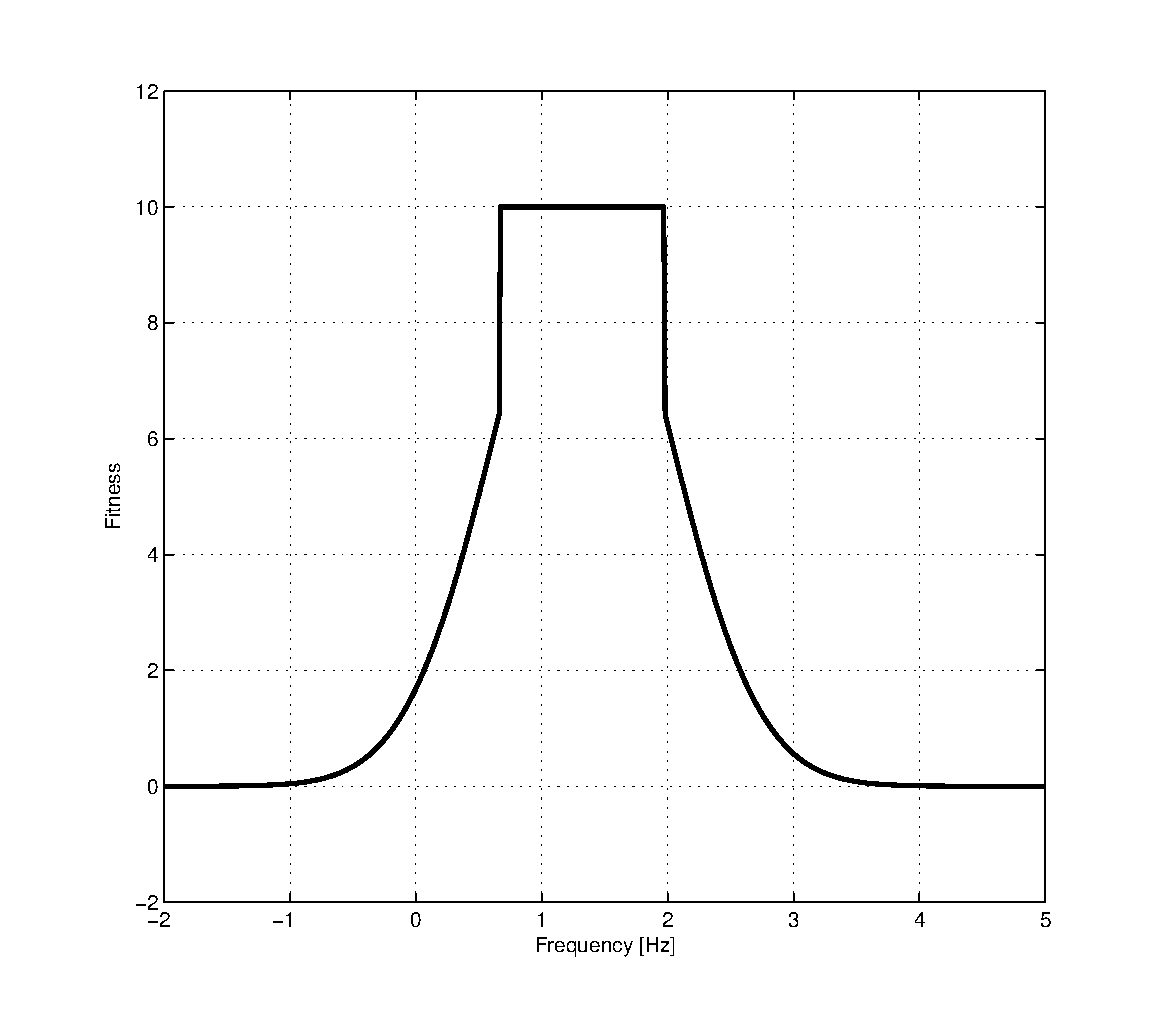
\includegraphics[width=\textwidth]{fig/FITNESS_FREC.eps}
        \caption{Funci�n de desempe�o de la frecuencia.}
        \label{fig:fitnessfrec}
    \end{subfigure}
    ~
    \begin{subfigure}[b]{0.48\textwidth}
    	\centering
        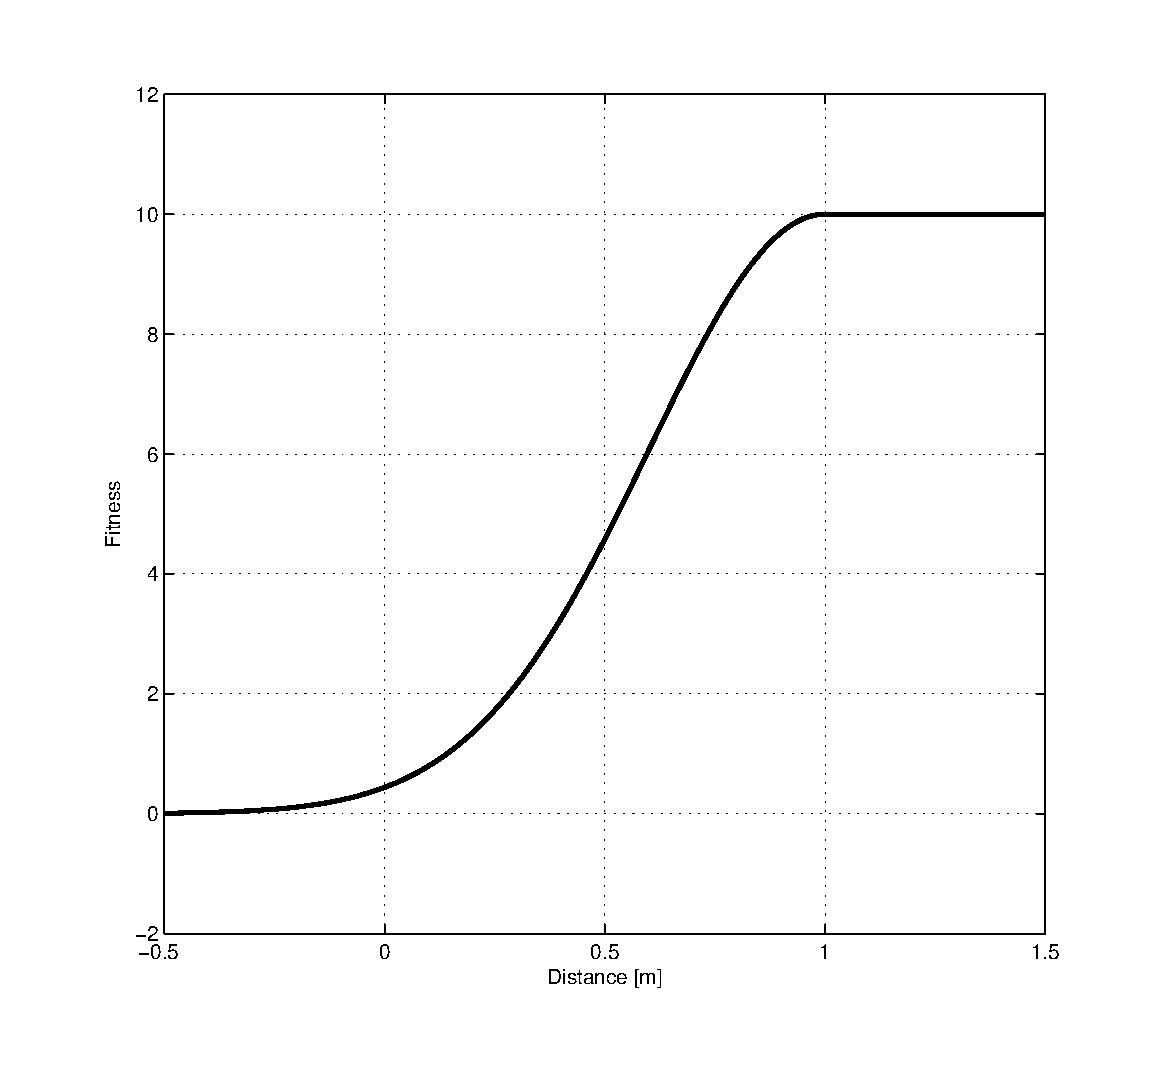
\includegraphics[width=\textwidth]{fig/FITNESS_DIST.eps}
        \caption{Funci�n de desempe�o de la distancia.}
        \label{fig:fitnessdist}
    \end{subfigure}
    \caption{\textbf{Funciones de desempe�o del entrenamiento.} En esta figura se muestran las funciones de desempe�o usadas para calificar que tan exitosa fue una caminata en el entrenamiento.}
    \label{fig:fitness}
\end{figure}

La distancia final alcanzada por el robot durante la simulaci�n es calculada por la diferencia de distancia entre el punto donde se posiciona el robot en el segundo uno de simulaci�n y el punto final que alcanza. Luego dicha distancia es ingresada a la funci�n del c�lculo del desempe�o de la caminata seg�n la distancia alcanzada, mostrada en la figura \ref{fig:fitnessdist}.

El resultado final del desempe�o de la caminata de un robot durante una simulaci�n estar� dado por una funci�n multi-objetivo compuesta por las dos funciones mostradas anteriormente, en donde prevalecer� el menor resultado entre ellas con el fin de evolucionar las CPPNs forzando a mejorar siempre el resultado de la variable con m�s problemas. As� si el desempe�o de la frecuencia y la distancia, por ejemplo, da como resultado 6 y 4 respectivamente, el desempe�o final del robot ser� de 4. Finalmente, el resultado obtenido ser� asignado a la red CPPN usada en la respectiva simulaci�n. Una vez comprendido el funcionamiento de cada simulaci�n y el c�lculo del desempe�o en cada una de estas es posible entender la estructura b�sica de un entrenamiento, como se muestra en la siguiente secci�n.

\section{ESTRUCTURA B�SICA DE UN ENTRENAMIENTO}

Un entrenamiento comienza con una poblaci�n o grupo inicial de CPPNs, cuyo n�mero es indicado por el usuario con anterioridad, conformando la primera generaci�n de redes a entrenar. Cada una de estas redes crear� un patr�n de conectividad en el substrato de HyperNEAT y \(\tau\)-HyperNEAT y se probar� en una simulaci�n para medir su desempe�o. Una vez que se midieron y evaluaron todas las CPPNs de la primera generaci�n deber�n evolucionar en una nueva generaci�n de redes CPPN, a trav�s del m�todo NEAT usado en ambos m�todos, del mismo tama�o de la poblaci�n inicial. Las CPPNs que conforman esta nueva generaci�n deber�n ser nuevamente probadas y evaluadas seg�n su desempe�o para dar origen a la generaci�n siguiente. Esto debe realizarse tantas veces como generaciones haya establecido el usuario para el entrenamiento dado. De esta forma si el usuario, por ejemplo, defini� al inicio del entrenamiento un n�mero de 100 generaciones con una poblaci�n de 100 CPPNs por generaci�n, el entrenamiento finalizar� una vez probadas las 10 mil CPPNs que conforman la totalidad de las generaciones. El proceso descrito anteriormente es la base de todo entrenamiento usando los m�todos HyperNEAT y \(\tau\)-HyperNEAT para cualquier experimento dado. En la secci�n siguiente se ahondar� en el funcionamiento del programa de entrenamiento, escrito en lenguaje C/C++, que hace uso de las herramientas presentadas anteriormente para generar caminatas en robots con extremidades m�viles.

\section{PROGRAMA DE ENTRENAMIENTO}

Una de las grandes problem�ticas presentes en los entrenamientos que comprometen periodos de tiempo real para su ejecuci�n es la extensa duraci�n de estos. El entrenamiento para la generaci�n de caminatas en robots con extremidades m�viles es uno de estos, ya que cada una de las simulaciones del entrenamiento debe durar los 6 segundos definidos para esta. As�, si un entrenamiento esta estipulado para evolucionar una poblaci�n de 100 CPPNs durante 100 generaciones, el tiempo estimado para su realizaci�n sobrepasa las 16 horas.

Debido a esta raz�n es que el programa de entrenamiento tiene la posibilidad de usar hebras (thread en ingles) para acelerar su ejecuci�n. El uso de hebras permitir� disminuir el tiempo total usado para el entrenamiento, ya que de esta forma ser� posible utilizar simult�neamente tantos simuladores como hebras corra el programa \footnote{Si bien una computadora actual puede ejecutar una gran cantidad de hebras simult�neamente, no podr� ejecutar la misma cantidad de simuladores debido a que la demanda de recursos generada por estos es elevada.}. De esta forma si el usuario, por ejemplo, indica el uso de 2 hebras, la poblaci�n de cada generaci�n ser� dividida en 2, ejecutando cada grupo de CPPNs en un simulador distinto y dividiendo el tiempo de entrenamiento a la mitad.

Una vez iniciado el programa de entrenamiento, este crear� todos los objetos necesarios para controlar al robot a usar dentro del simulador, usando la ya mencionada librer�a RobotLib. De usar m�s de un simulador, se deber�n crear tantos objetos repetidos como simuladores se ejecuten. Tambi�n se deben crear los objetos correspondientes al m�todo a utilizar (HyperNEAT o \(\tau\)-HyperNEAT), que al igual que en el caso de RobotLib, deben corresponder en n�mero a la cantidad de simuladores o hebras estipuladas para el entrenamiento.

Ya creadas todas las entidades necesarias para el funcionamiento de los m�todos de neuroevoluci�n y de los simuladores el programa continuar� con un bucle for que iterar� tantas veces como generaciones se hayan estipulado para el entrenamiento, y en cada ciclo de este se iniciar�n las hebras que se dividir�n la poblaci�n de CPPNs para ejecutar las simulaciones correspondientes a cada una de ellas. Luego que cada una de las hebras termine de probar y evaluar cada unas de las CPPNs asignadas, estas terminar�n su ejecuci�n volviendo el programa al bucle for para posteriormente evolucionar la poblaci�n de CPPNs en una nueva generaci�n y completar nuevamente un nuevo ciclo del bucle. Una vez realizados todos los ciclos del bucle for se obtendr� la red CPPN capaz de crear el patr�n de conectividad m�s adecuado sobre el substrato del m�todo usado, logrando la caminata con el mejor desempe�o del entrenamiento.

Para comprobar el funcionamiento de HyperNEAT y \(\tau\)-HyperNEAT en la generaci�n de caminatas en robots con extremidades m�viles se entrenar�n a 3 robots distintos: Quadratot, ArgoV2 y Rosita (ver Figura \ref{fig:robots}), siendo el primero un robot dise�ado por el Investigador de la Universidad de Chile Juan Crist�bal Zagal, con el objeto de ser usado para comprobar el funcionamiento de distintos m�todos para la generaci�n de caminatas; y los �ltimos dos, robots dise�ados por el estudiante de Ingenier�a en Dise�o de Productos Cristian Osorio M�ndez para el Departamento de Electr�nica de La Universidad T�cnica Federico Santa Mar�a. En la secci�n siguiente se mostrar�n los resultados de los entrenamientos realizados sobre cada uno de estos robots usando ambos m�todos de neuroevoluci�n. Todos los c�digos utilizados en la siguiente secci�n pueden ser descargados desde el repositorio Github \url{https://github.com/osilvam/Memoria} y probados de manera f�cil y sencilla.

\section{RESULTADOS DE LOS ENTRENAMIENTOS}

Tal como se mencion� anteriormente, los entrenamientos para la generaci�n de caminatas usando los m�todos de neuroevoluci�n HyperNEAT y \(\tau\)-HyperNEAT se aplicar�n en 3 plataformas rob�ticas, Quadratot, ArgoV2 y Rosita. A continuaci�n se mostrar�n los resultados obtenidos para cada una de ellas.

\subsection{QUADRATOT}

A continuaci�n se presentaran los resultados de los entrenamientos para la generaci�n de caminatas realizados sobre la plataforma rob�tica Quadratot con el fin de identificar avances entre el desempe�o de la tarea al usar el m�todo HyperNEAT y el nuevo m�todo \(\tau\)-HyperNEAT. 

En la figura \ref{fig:quadratot_fitness} se muestra un gr�fico comparativo entre el desempe�o del m�todo HyperNEAT y \(\tau\)-HyperNEAT, siendo cada una de las curvas el promedio de un gran n�mero de entrenamientos. Como se puede apreciar, en t�rminos de resultados num�ricos, no existe mayor diferencia entre los m�todos, alcanzando ambos un promedio de desempe�o generacional cercano a 5 de 10, con una peque�a diferencia en la rapidez en el progreso al inicio de los entrenamientos. Adem�s, la magnitud de la dispersi�n del desempe�o obtenido para ambos m�todos se mantiene.

\begin{figure}[ht!]
	\centering
	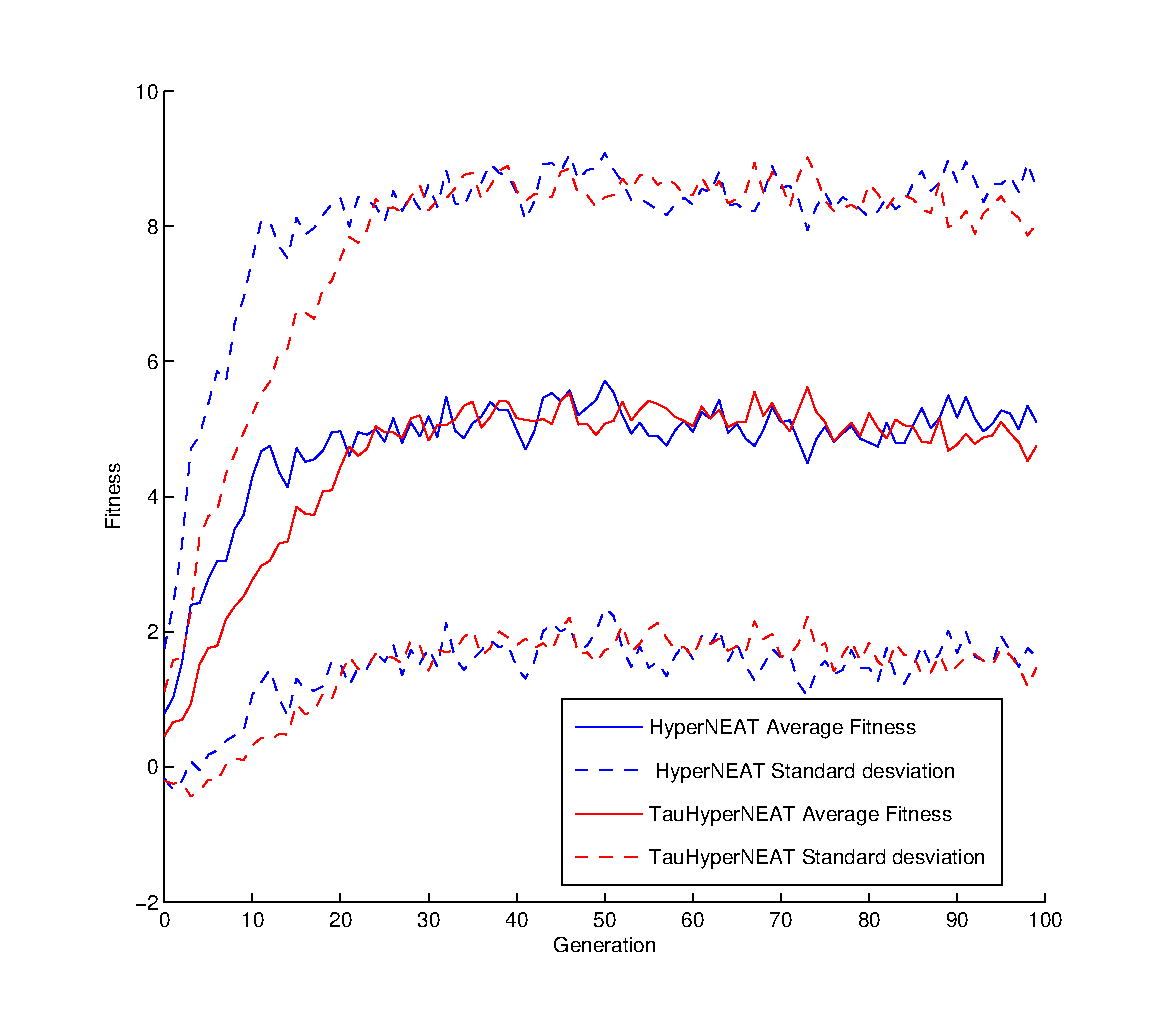
\includegraphics[width=0.75\textwidth]{fig/QUADRATOT_FITNESS.eps}
    \caption{\textbf{Gr�fico comparativo del desempe�o entre HyperNEAT y \(\tau\)-HyperNEAT.} En esta figura puede observarse la gran similitud en el desempe�o promedio obtenido de entrenamientos de generaci�n de caminatas sobre el robot Quadratot usando ambos m�todos.}
    \label{fig:quadratot_fitness}	
\end{figure}

\begin{figure}[ht!]
	\centering
	\begin{subfigure}[b]{\textwidth}
		\centering
        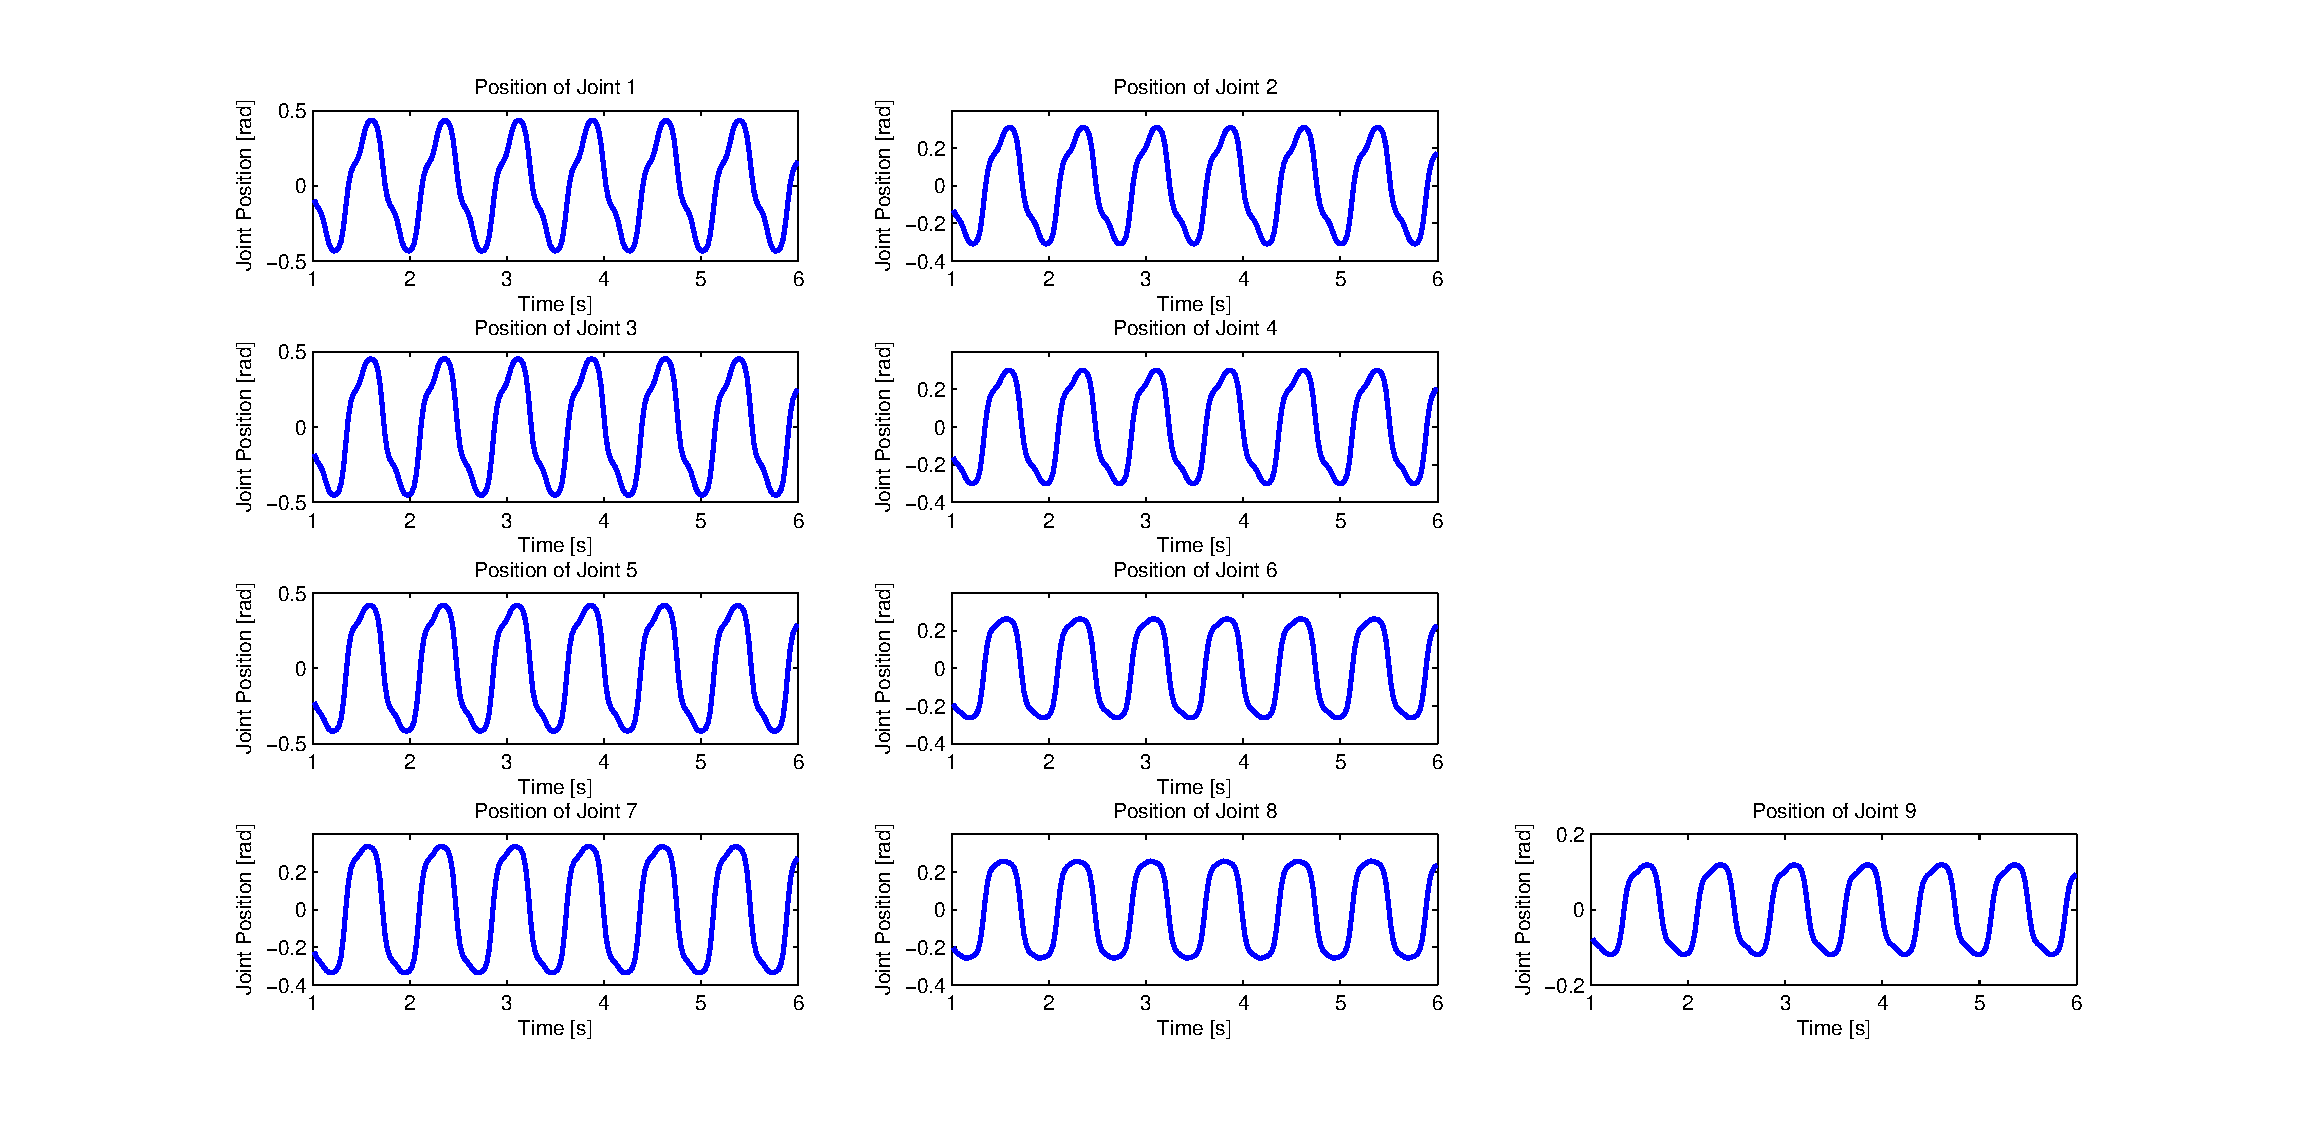
\includegraphics[width=\textwidth]{fig/QUADRATOT_JP_HYPERNEAT.eps}
        \caption{HyperNEAT.}
        \label{fig:quadratot_jp_hyperneat}
    \end{subfigure}
    
    \begin{subfigure}[b]{\textwidth}
    	\centering
        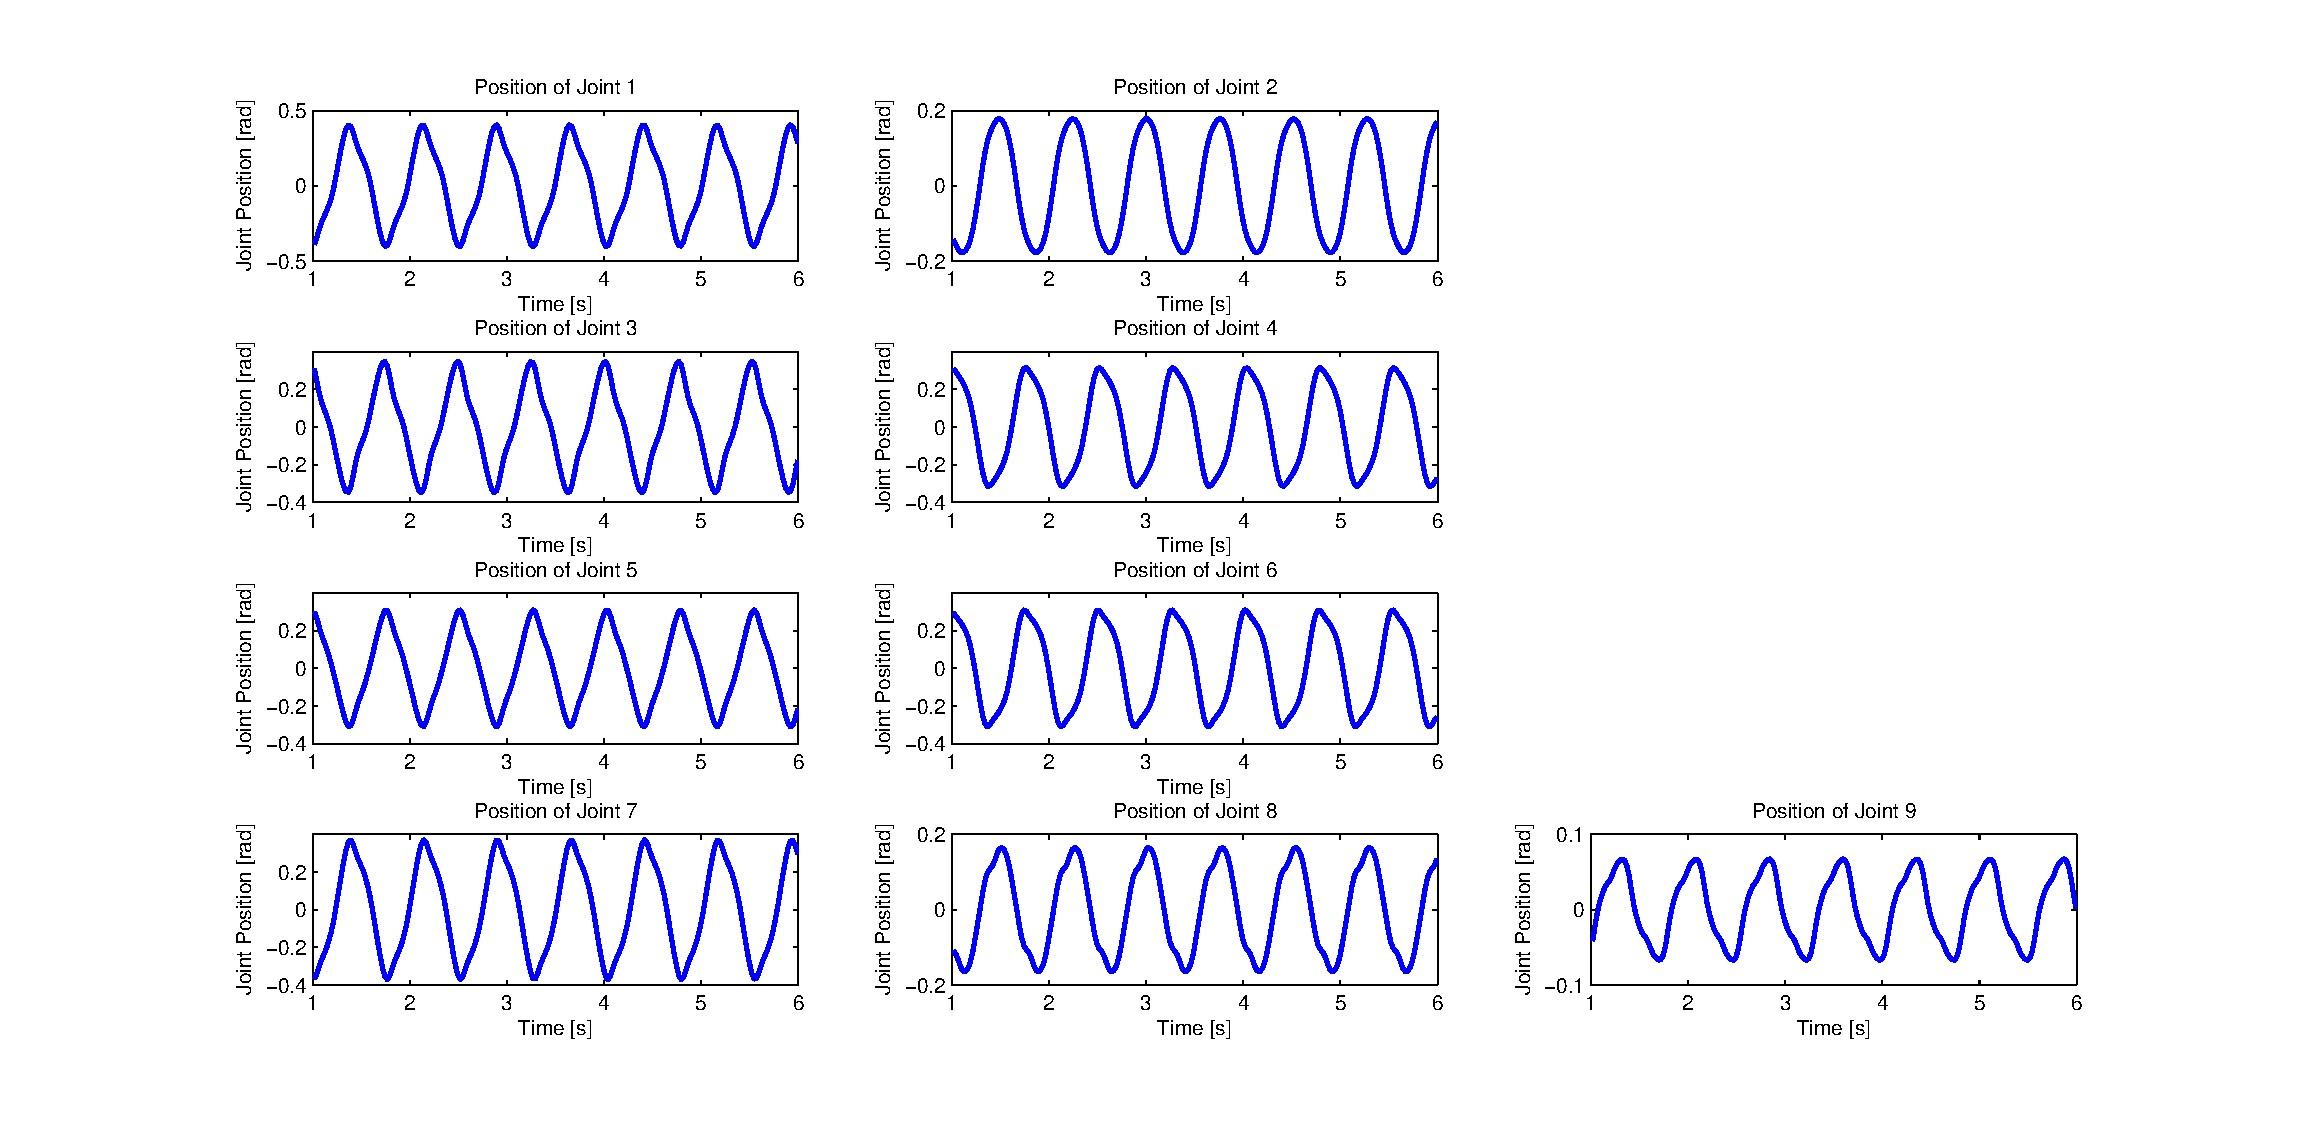
\includegraphics[width=\textwidth]{fig/QUADRATOT_JP_TAUHYPERNEAT.eps}
        \caption{\(\tau\)-HyperNEAT.}
        \label{fig:quadratot_jp_tauhyperneat}
    \end{subfigure}
    \caption{\textbf{Posici�n de los motores de Quadratot dada por HyperNEAT y \(\tau\)-HyperNEAT.} En la figura se muestran los gr�ficos de las se�ales entregadas a los motores del robot Quadratot en caminatas representativas realizadas usando el m�todo HyperNEAT (a) y el nuevo m�todo \(\tau\)-HyperNEAT (b). En ambos esquemas de gr�ficos, cada fila corresponde a una de las extremidades del robot, siendo la primera columna el motor m�s cercano al torso central, y la segunda columna el motor m�s alejado. El gr�fico solitario de la columna 3 corresponde al motor ubicado entre los torsos centrales del robot.}
    \label{fig:quadratot_jp}
\end{figure}

\clearpage

Sin embargo, a pesar de que num�ricamente no exista gran mejora entre el m�todo propuesto y su predecesor, si la hay en t�rminos de la ejecuci�n misma de las caminatas logradas por estos. En la figura \ref{fig:quadratot_jp} se pueden observar gr�ficos de las se�ales entregadas a los motores por ambos m�todos, siendo los dos set de gr�ficos mostrados, resultados representativos para cada m�todo. En el esquema de gr�ficos, las dos primeras columnas de cada fila corresponden a las se�ales dadas a los motores de una extremidad de Quadratot. El gr�fico restante de la tercera columna corresponde al grado de libertad que une las dos piezas que componen el torso central de Quadratot. Se puede apreciar en la figura \ref{fig:quadratot_jp_hyperneat} que todas las se�ales dadas a los motores de Quadratot poseen la misma fase, a diferencia de la figura \ref{fig:quadratot_jp_tauhyperneat}, en la que se ven claramente diferencias de fases en las se�ales de los motores por cada par de extremidades, implicando que el movimiento de estas para el caso de HyperNEAT fuera el mismo a cada momento y que para el caso de \(\tau\)-HyperNEAT fuera alternado, estirando y contrayendo sus pares de extremidades a distintos tiempos.

Adem�s de la diferencia en la fase de las se�ales de los motores en sus extremidades, Quadratot presenta un desplazamiento m�s fluido y direccionado al momento de usar \(\tau\)-HyperNEAT para la generaci�n de las caminatas, como se ve en la figura \ref{fig:quadratot_p}, de la que se infiere que al usar \(\tau\)-HyperNEAT el robot avanz� con una trayectoria totalmente recta y fluida (figura \ref{fig:quadratot_p_tauhyperneat}), a diferencia del caso usar HyperNEAT, en donde su trayectoria fue turbulenta y poco lineal (figura \ref{fig:quadratot_p_hyperneat}). M�s aun, las caracter�sticas estrictamente lineales en el desplazamiento de Quadratot al usar \(\tau\)-HyperNEAT, en conjunto con la informaci�n entregada por el cuarto gr�fico del set indican que el desplazamiento del robot, adem�s de poseer una trayectoria lineal se realiza a una velocidad constante en el tiempo.

\begin{figure}[ht!]
	\centering
	\begin{subfigure}[b]{\textwidth}
		\centering
        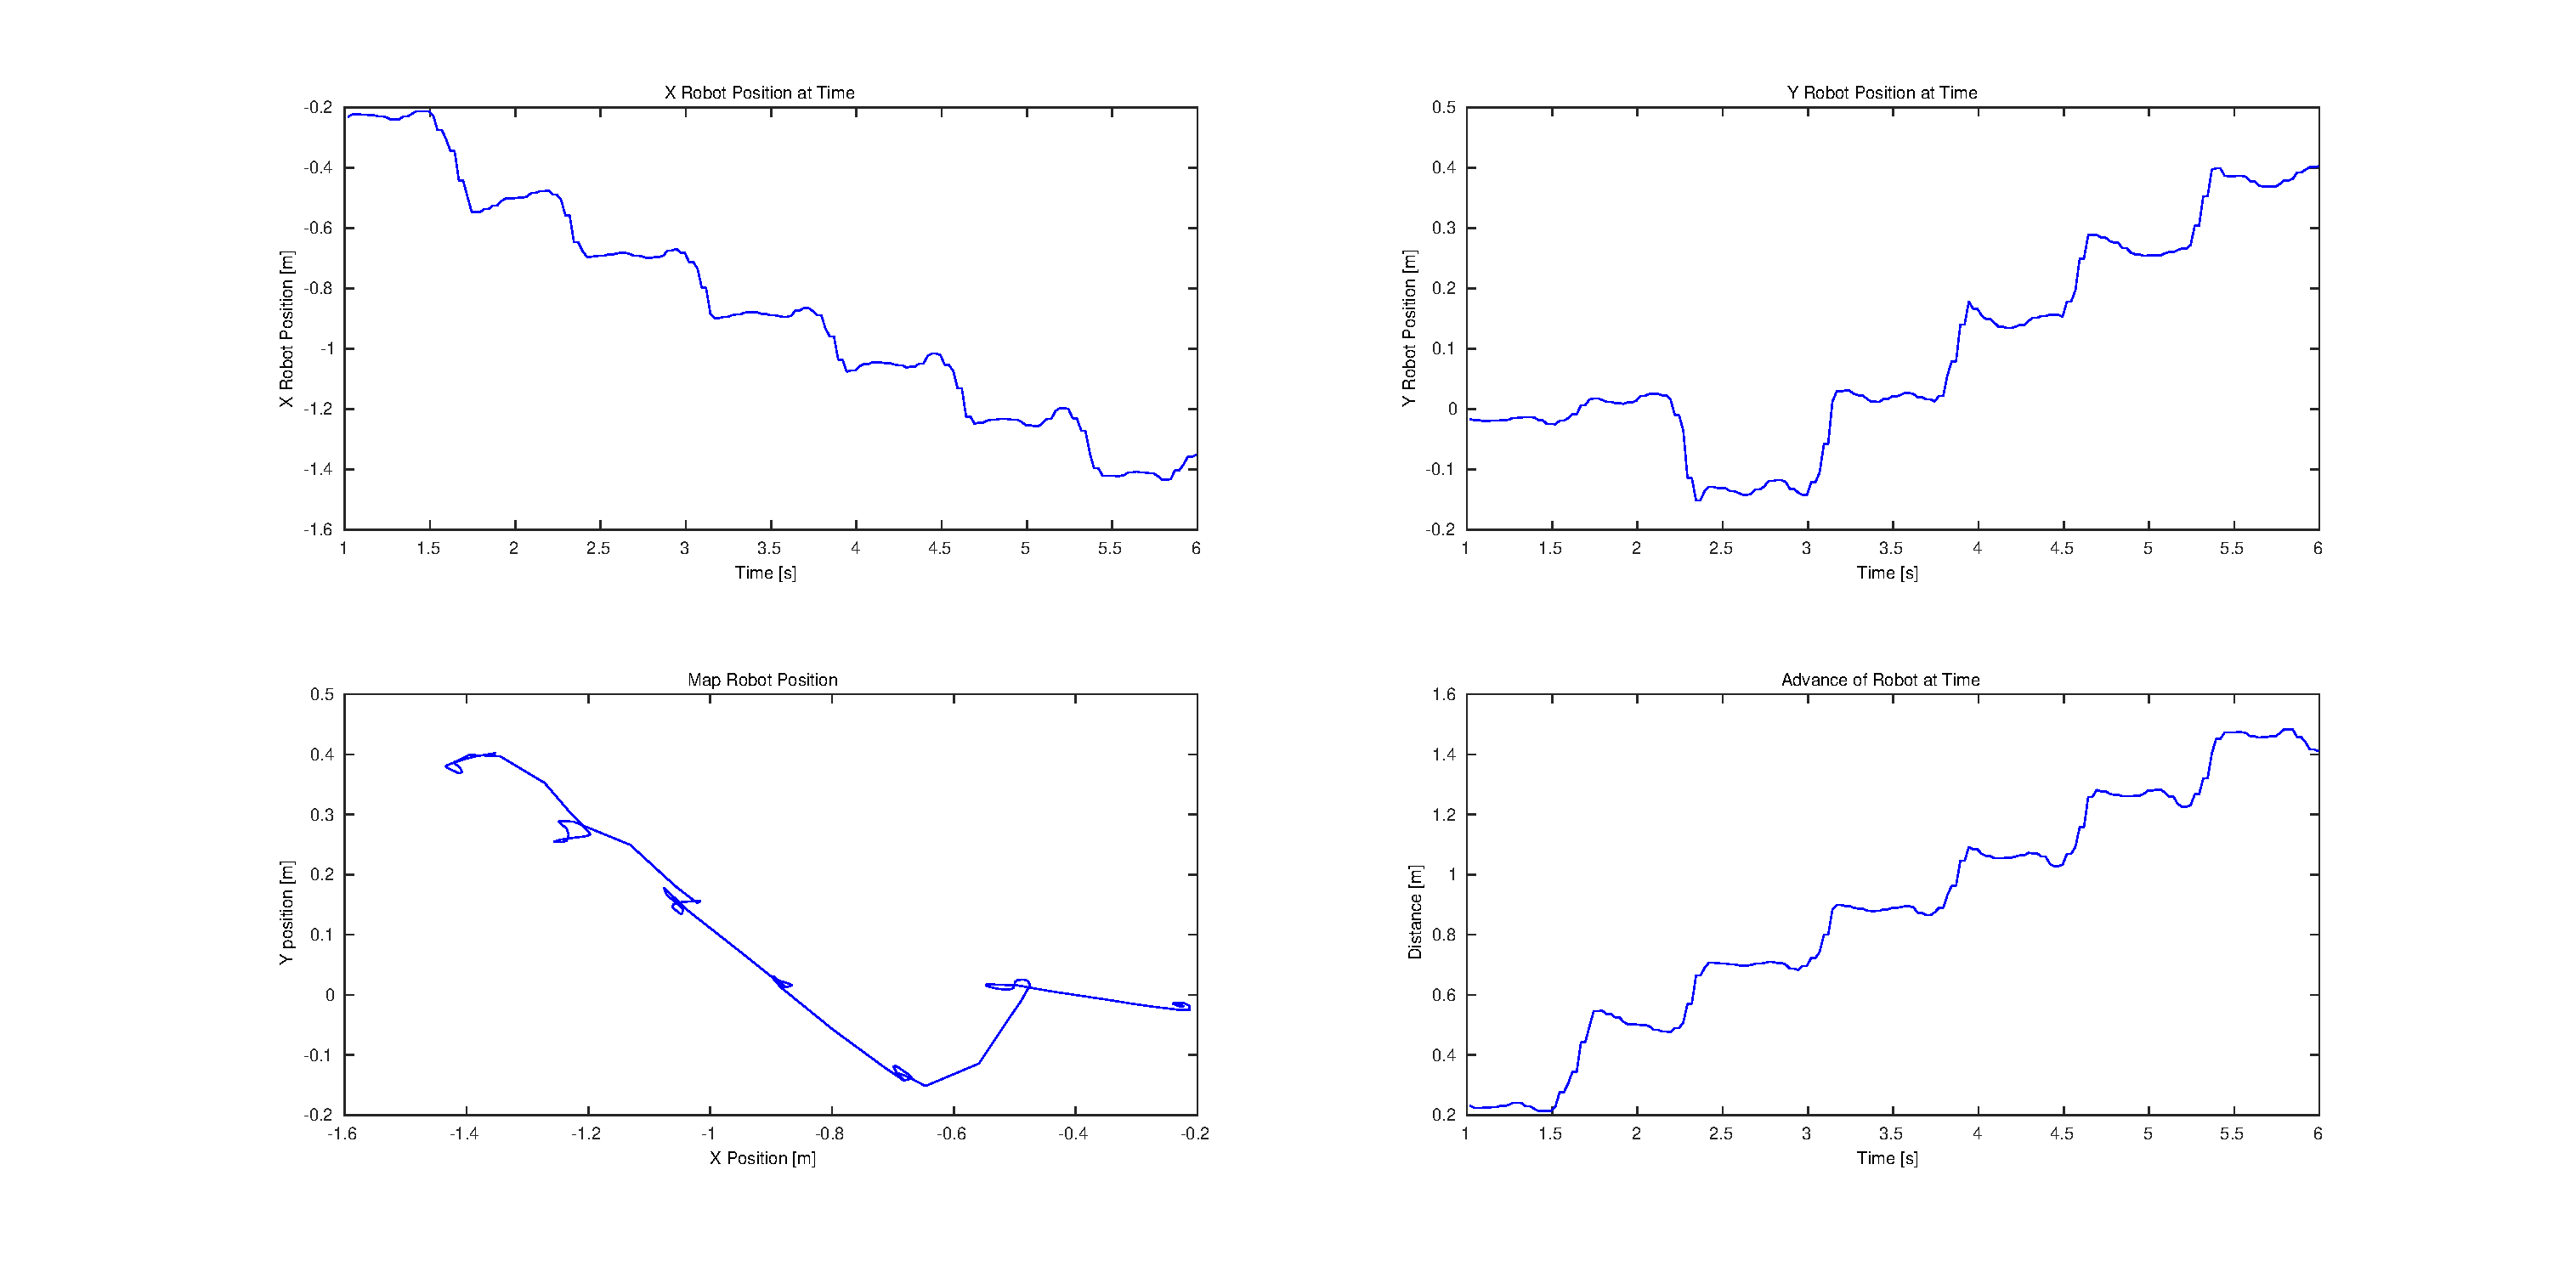
\includegraphics[width=\textwidth]{fig/QUADRATOT_POSITION_HYPERNEAT.eps}
        \caption{HyperNEAT.}
        \label{fig:quadratot_p_hyperneat}
    \end{subfigure}
    
    \begin{subfigure}[b]{\textwidth}
    	\centering
        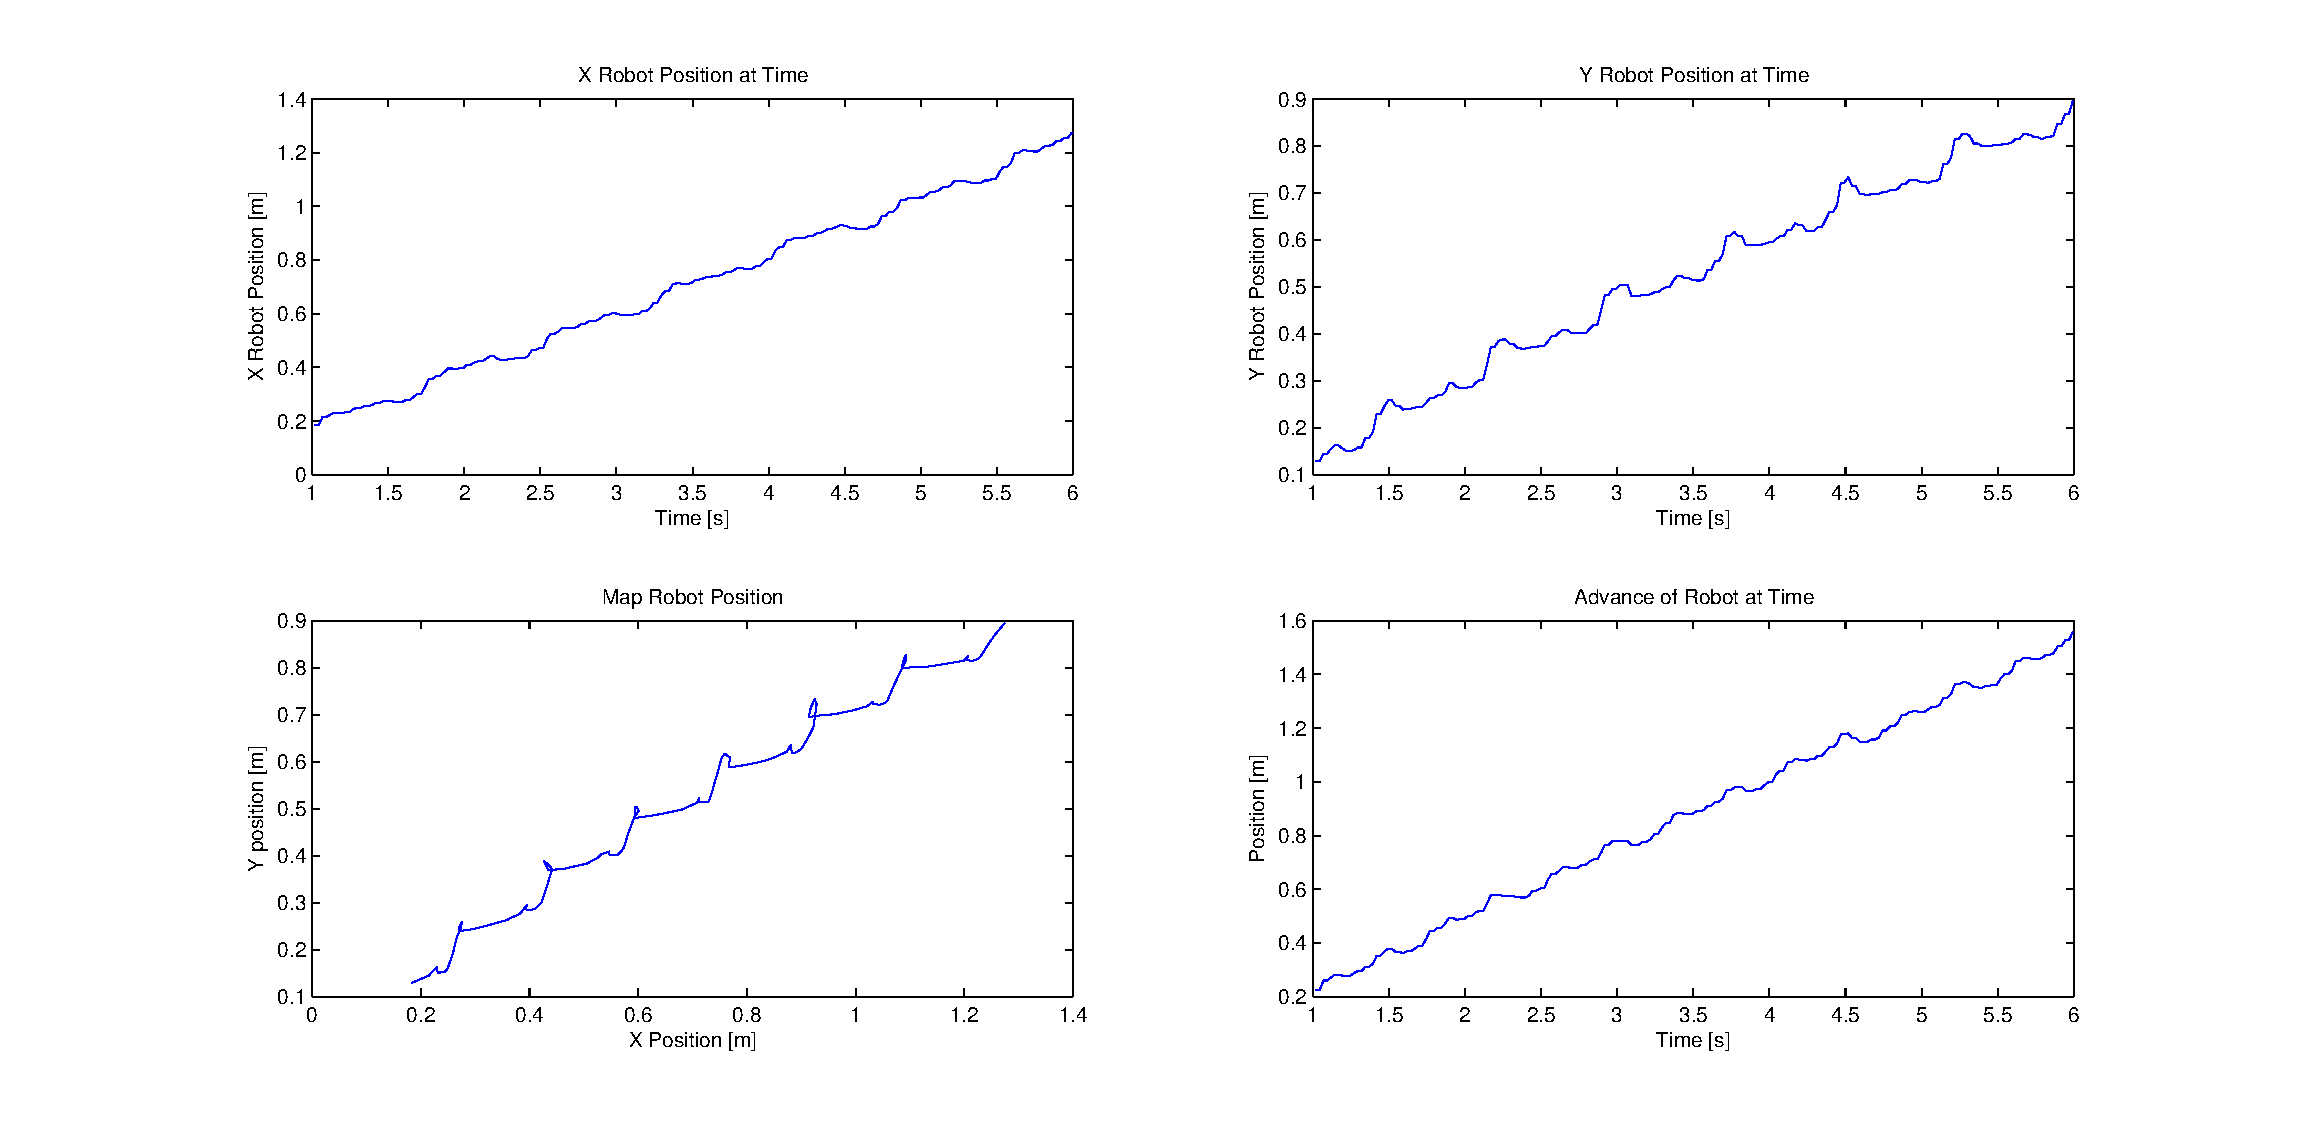
\includegraphics[width=\textwidth]{fig/QUADRATOT_POSITION_TAUHYPERNEAT.eps}
        \caption{\(\tau\)-HyperNEAT.}
        \label{fig:quadratot_p_tauhyperneat}
    \end{subfigure}
    \caption{\textbf{Desplazamiento de Quadratot en el escenario dado por HyperNEAT y \(\tau\)-HyperNEAT.} Los sets de gr�ficos presentes en esta figura muestran el desplazamiento de Quadratot a lo largo del escenario de simulaci�n en distintas medidas. Los gr�ficos superiores izquierdo y derecho muestra el desplazamiento en el tiempo del robot a lo largo del los ejes $x$ e $y$ respectivamente. EL gr�fico inferior izquierdo corresponde al desplazamiento del robot a lo largo del plano $xy$ del escenario. Finalmente el gr�fico inferior derecho corresponde a la distancia recta medida del robot hacia el punto de partida del escenario en el tiempo.}
    \label{fig:quadratot_p}
\end{figure}

\clearpage

\subsection{ARGOV2}

A continuaci�n se presentaran los resultados de los entrenamientos para la generaci�n de caminatas realizados sobre la plataforma rob�tica ArgoV2 con el fin de identificar avances entre el desempe�o de la tarea al usar el m�todo HyperNEAT y el nuevo m�todo \(\tau\)-HyperNEAT. 

En la figura \ref{fig:argov2_fitness} se muestra un gr�fico comparativo entre el desempe�o del m�todo HyperNEAT y \(\tau\)-HyperNEAT, siendo cada una de las curvas el promedio de un gran n�mero de entrenamientos. Como se puede apreciar al igual que en el caso de Quadratot, en t�rminos de resultados num�ricos, no existe mayor diferencia entre los m�todos (\(\tau\)-HyperNEAT solo supera apenas en 0.5 puntos de 10 a su predecesor), alcanzando ambos un promedio de desempe�o generacional tambi�n cercano al 5. Adem�s, la magnitud de la dispersi�n del desempe�o obtenido para ambos m�todos se mantiene.

\begin{figure}[ht!]
	\centering
	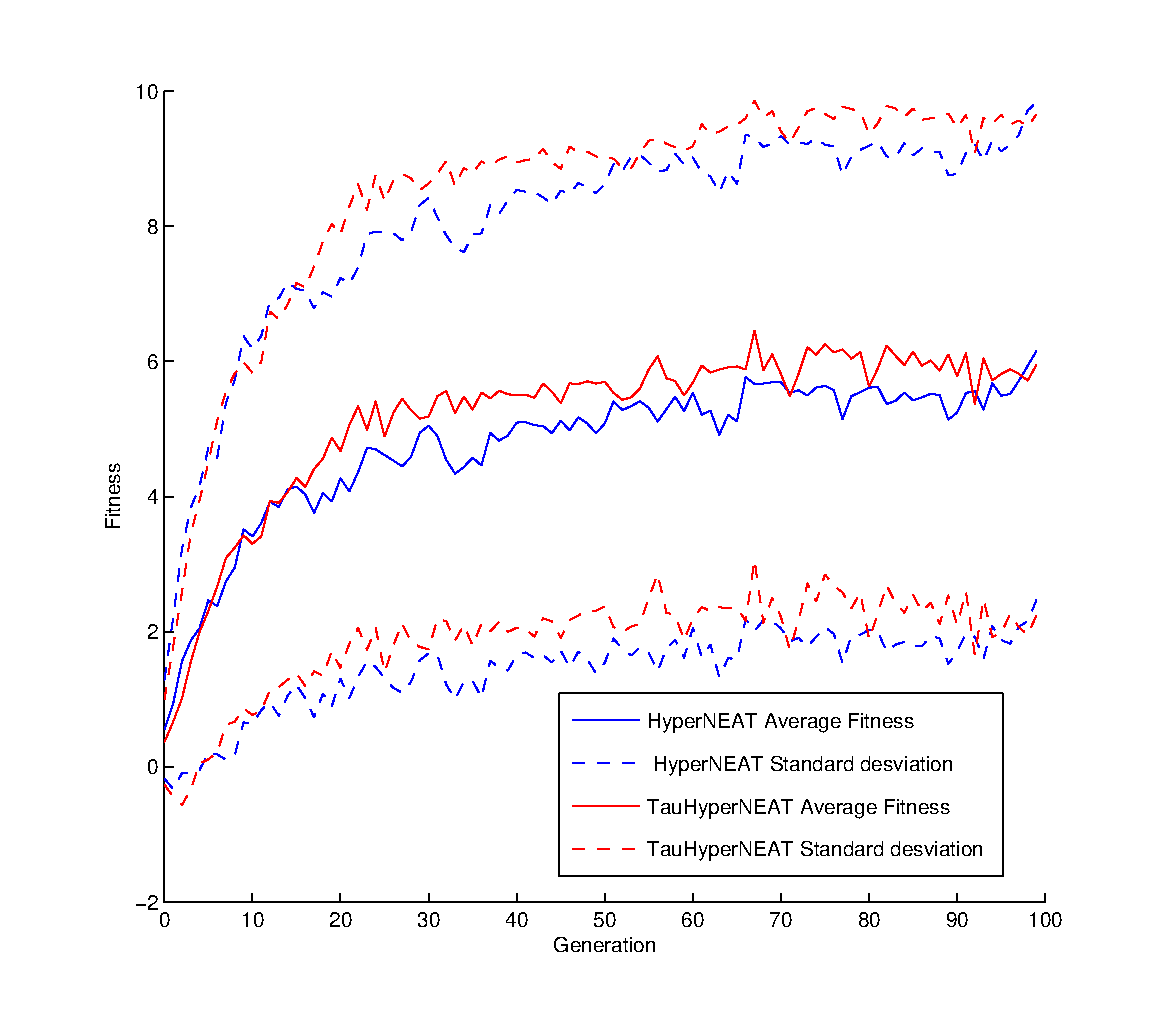
\includegraphics[width=0.75\textwidth]{fig/ARGOV2_FITNESS.eps}
    \caption{\textbf{Gr�fico comparativo del desempe�o entre HyperNEAT y \(\tau\)-HyperNEAT.} En esta figura puede observarse la poca diferencia en el desempe�o promedio obtenido de entrenamientos de generaci�n de caminatas sobre el robot ArgoV2 usando ambos m�todos.}
    \label{fig:argov2_fitness}	
\end{figure}

\begin{figure}[ht!]
	\centering
	\begin{subfigure}[b]{\textwidth}
		\centering
        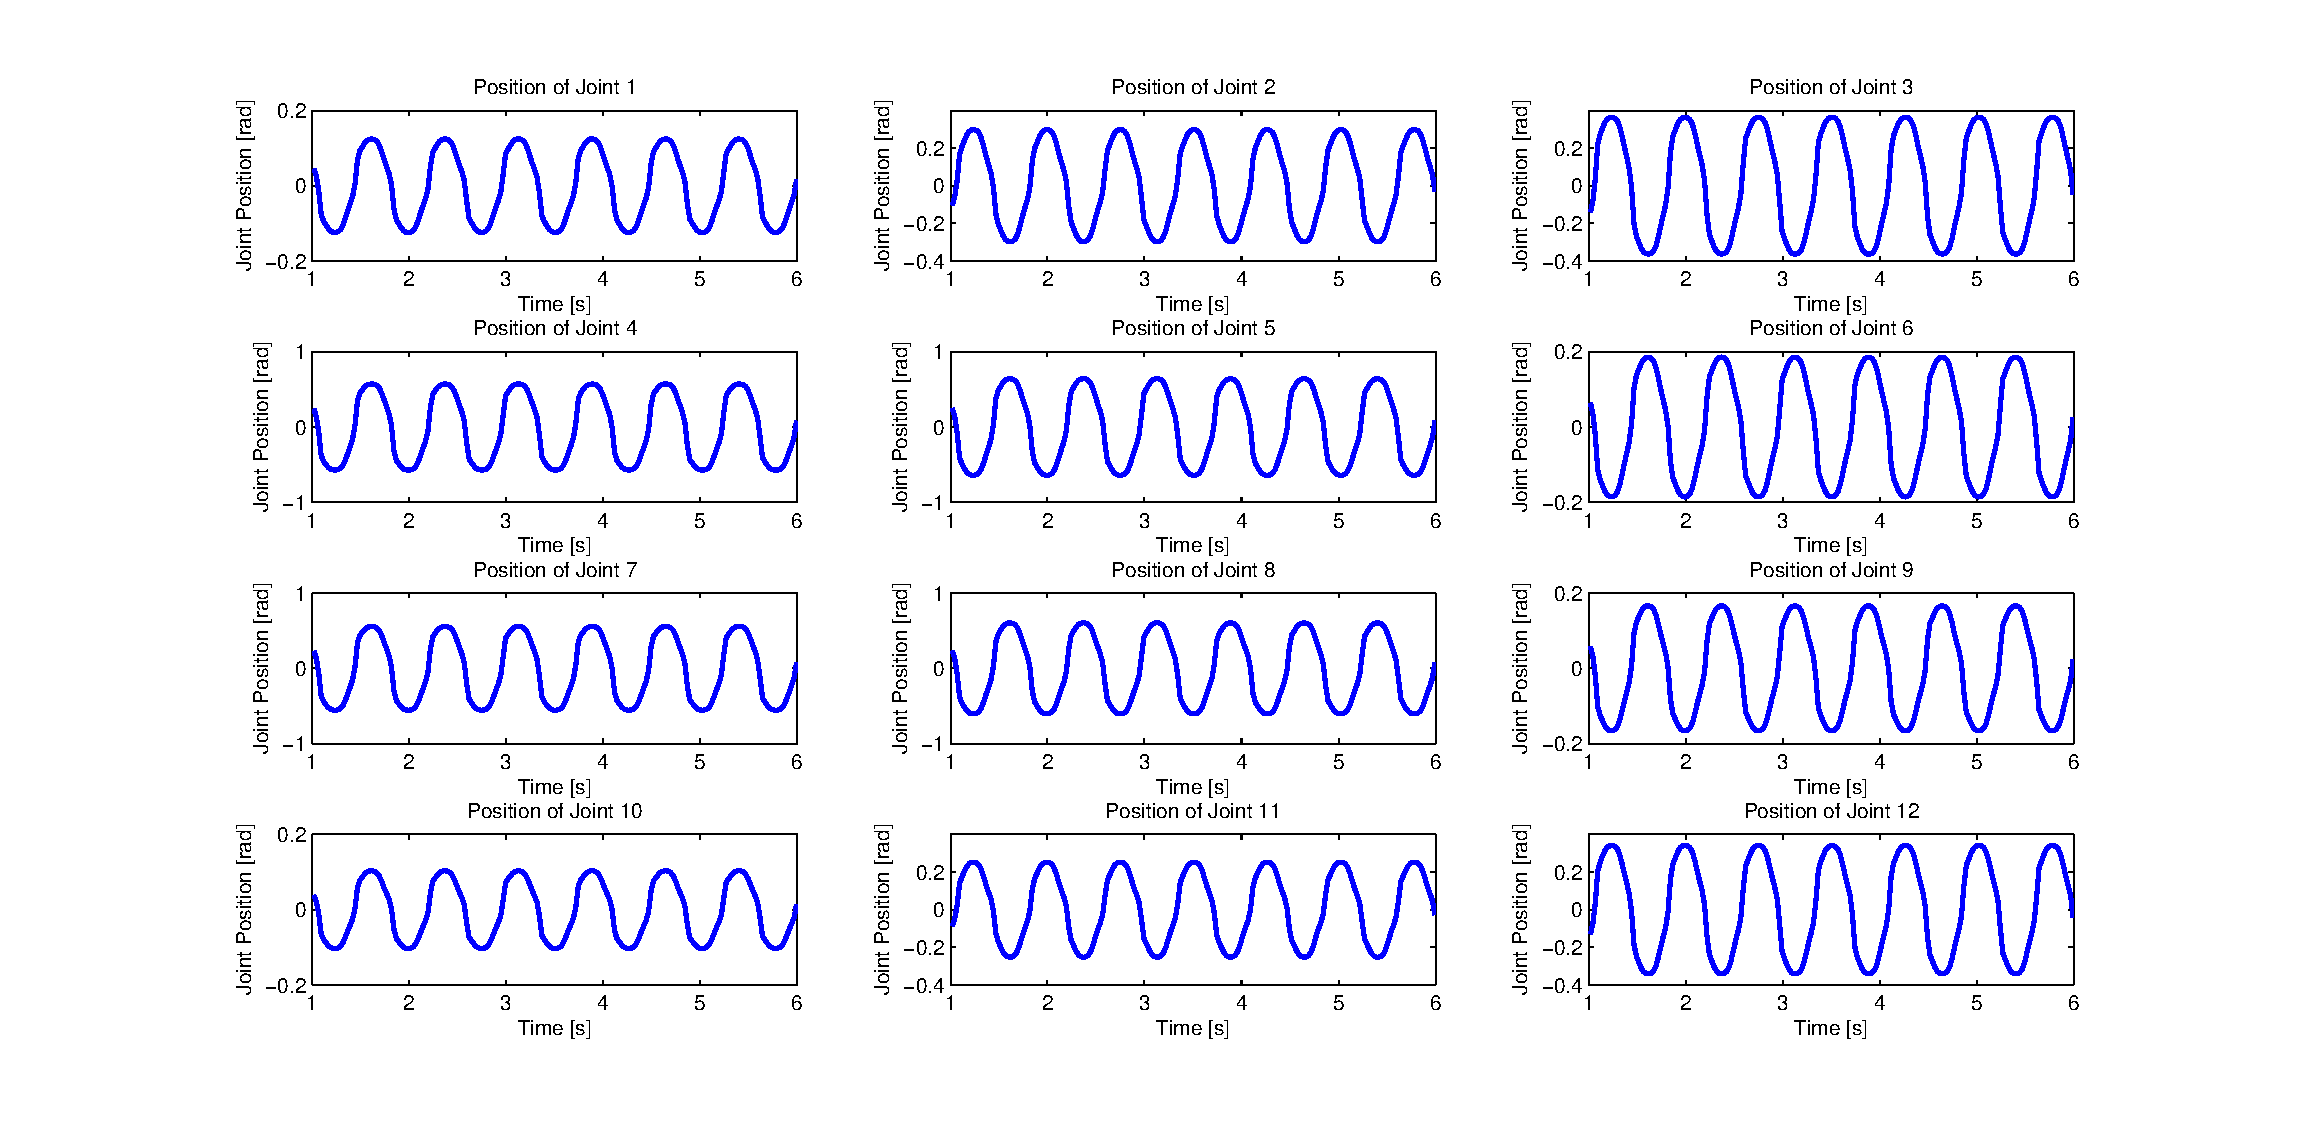
\includegraphics[width=\textwidth]{fig/ARGOV2_JP_HYPERNEAT.eps}
        \caption{HyperNEAT.}
        \label{fig:argov2_jp_hyperneat}
    \end{subfigure}
    
    \begin{subfigure}[b]{\textwidth}
    	\centering
        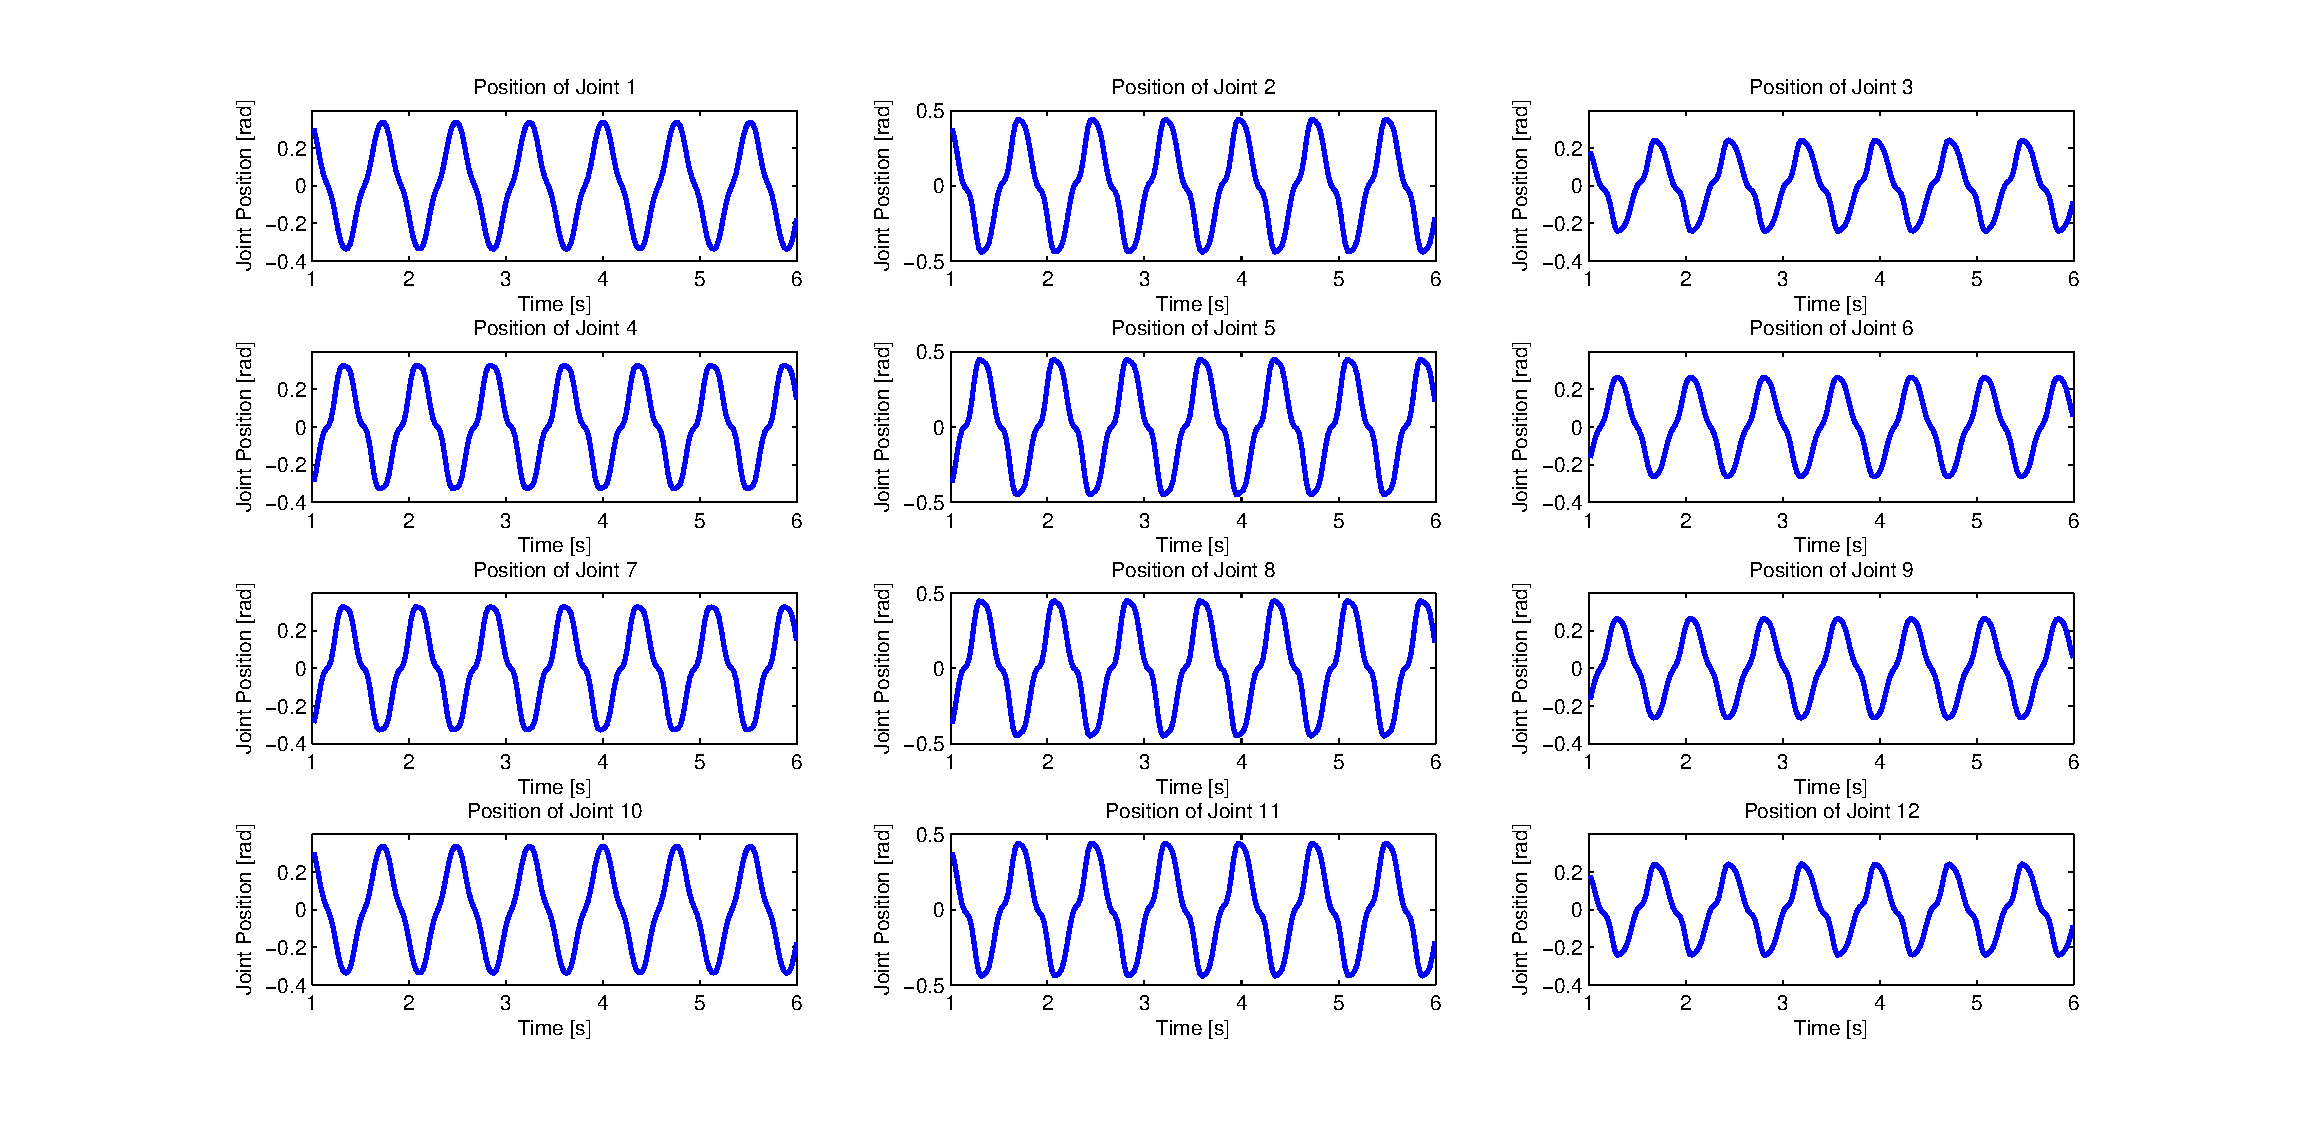
\includegraphics[width=\textwidth]{fig/ARGOV2_JP_TAUHYPERNEAT.eps}
        \caption{\(\tau\)-HyperNEAT.}
        \label{fig:argov2_jp_tauhyperneat}
    \end{subfigure}
     \caption{\textbf{Posici�n de los motores de ArgoV2 dada por HyperNEAT y \(\tau\)-HyperNEAT.} En la figura se muestran los gr�ficos de las se�ales entregadas a los motores del robot ArgoV2 en caminatas representativas realizadas usando el m�todo HyperNEAT (a) y el nuevo m�todo \(\tau\)-HyperNEAT (b). En ambos esquemas de gr�ficos, cada fila corresponde a una de las extremidades del robot, siendo la primera columna el motor m�s cercano al torso central, la segunda columna el motor intermedio de cada extremidad, y la tercera columna el motor mas alejado del torso.}
    \label{fig:argov2_jp}
\end{figure}

\clearpage

Tal como se di� en el caso de Quadratot, a pesar de que num�ricamente no exista una mejora substancial entre el m�todo propuesto y HyperNEAT, la hay en t�rminos de la ejecuci�n de las caminatas logradas. En la figura \ref{fig:argov2_jp} se pueden observar gr�ficos de las se�ales entregadas a los motores por ambos m�todos, siendo los dos set de gr�ficos mostrados, resultados representativos para cada m�todo. Se puede apreciar en la figura \ref{fig:argov2_jp_tauhyperneat}, al igual que en la figura \ref{fig:argov2_jp_tauhyperneat}, que existe una diferencia clara de fase, de aproximadamente $\pi$ radianes entre pares de extremidades. Si bien las se�ales del set de gr�ficos correspondiente al m�todo HyperNEAT tambi�n presentan desfases entre las distintas extremidades del robot, estos desfases no se manifiestan iguales a lo largo de ellas, existiendo distintas fases en las se�ales de los motores dados para una extremidad. Esto se observa en las extremidades 1 y 4 vistas de la figura \ref{fig:argov2_jp_hyperneat}, en donde el primer motor posee una fase retrasada en $\pi$ radianes en comparaci�n con los otros dos.

Adem�s de la diferencia en la fase de las se�ales de los motores en sus extremidades, ArgoV2 presenta un desplazamiento m�s fluido y con menos oscilaciones al momento de usar \(\tau\)-HyperNEAT para la generaci�n de las caminatas, como se ve en la figura \ref{fig:argov2_p}, de la que se infiere que al usar \(\tau\)-HyperNEAT el robot avanz� con una trayectoria lineal (figura \ref{fig:argov2_p_tauhyperneat}) con menos oscilaciones que al usar HyperNEAT, en donde su trayectoria fue m�s oscilante, pero aun as� recta (figura \ref{fig:quadratot_p_hyperneat}). Para el caso de esta plataforma rob�tica, ambos m�todos lograron realizar una trayectoria en promedio recta, y en conjunto con la informaci�n entregada por el cuarto gr�fico de cada set, se infiere que adem�s de haberse realizado trayectorias rectas, estas fueron realizadas a una velocidad constante en el tiempo.

\begin{figure}[ht!]
	\centering
	\begin{subfigure}[b]{\textwidth}
		\centering
        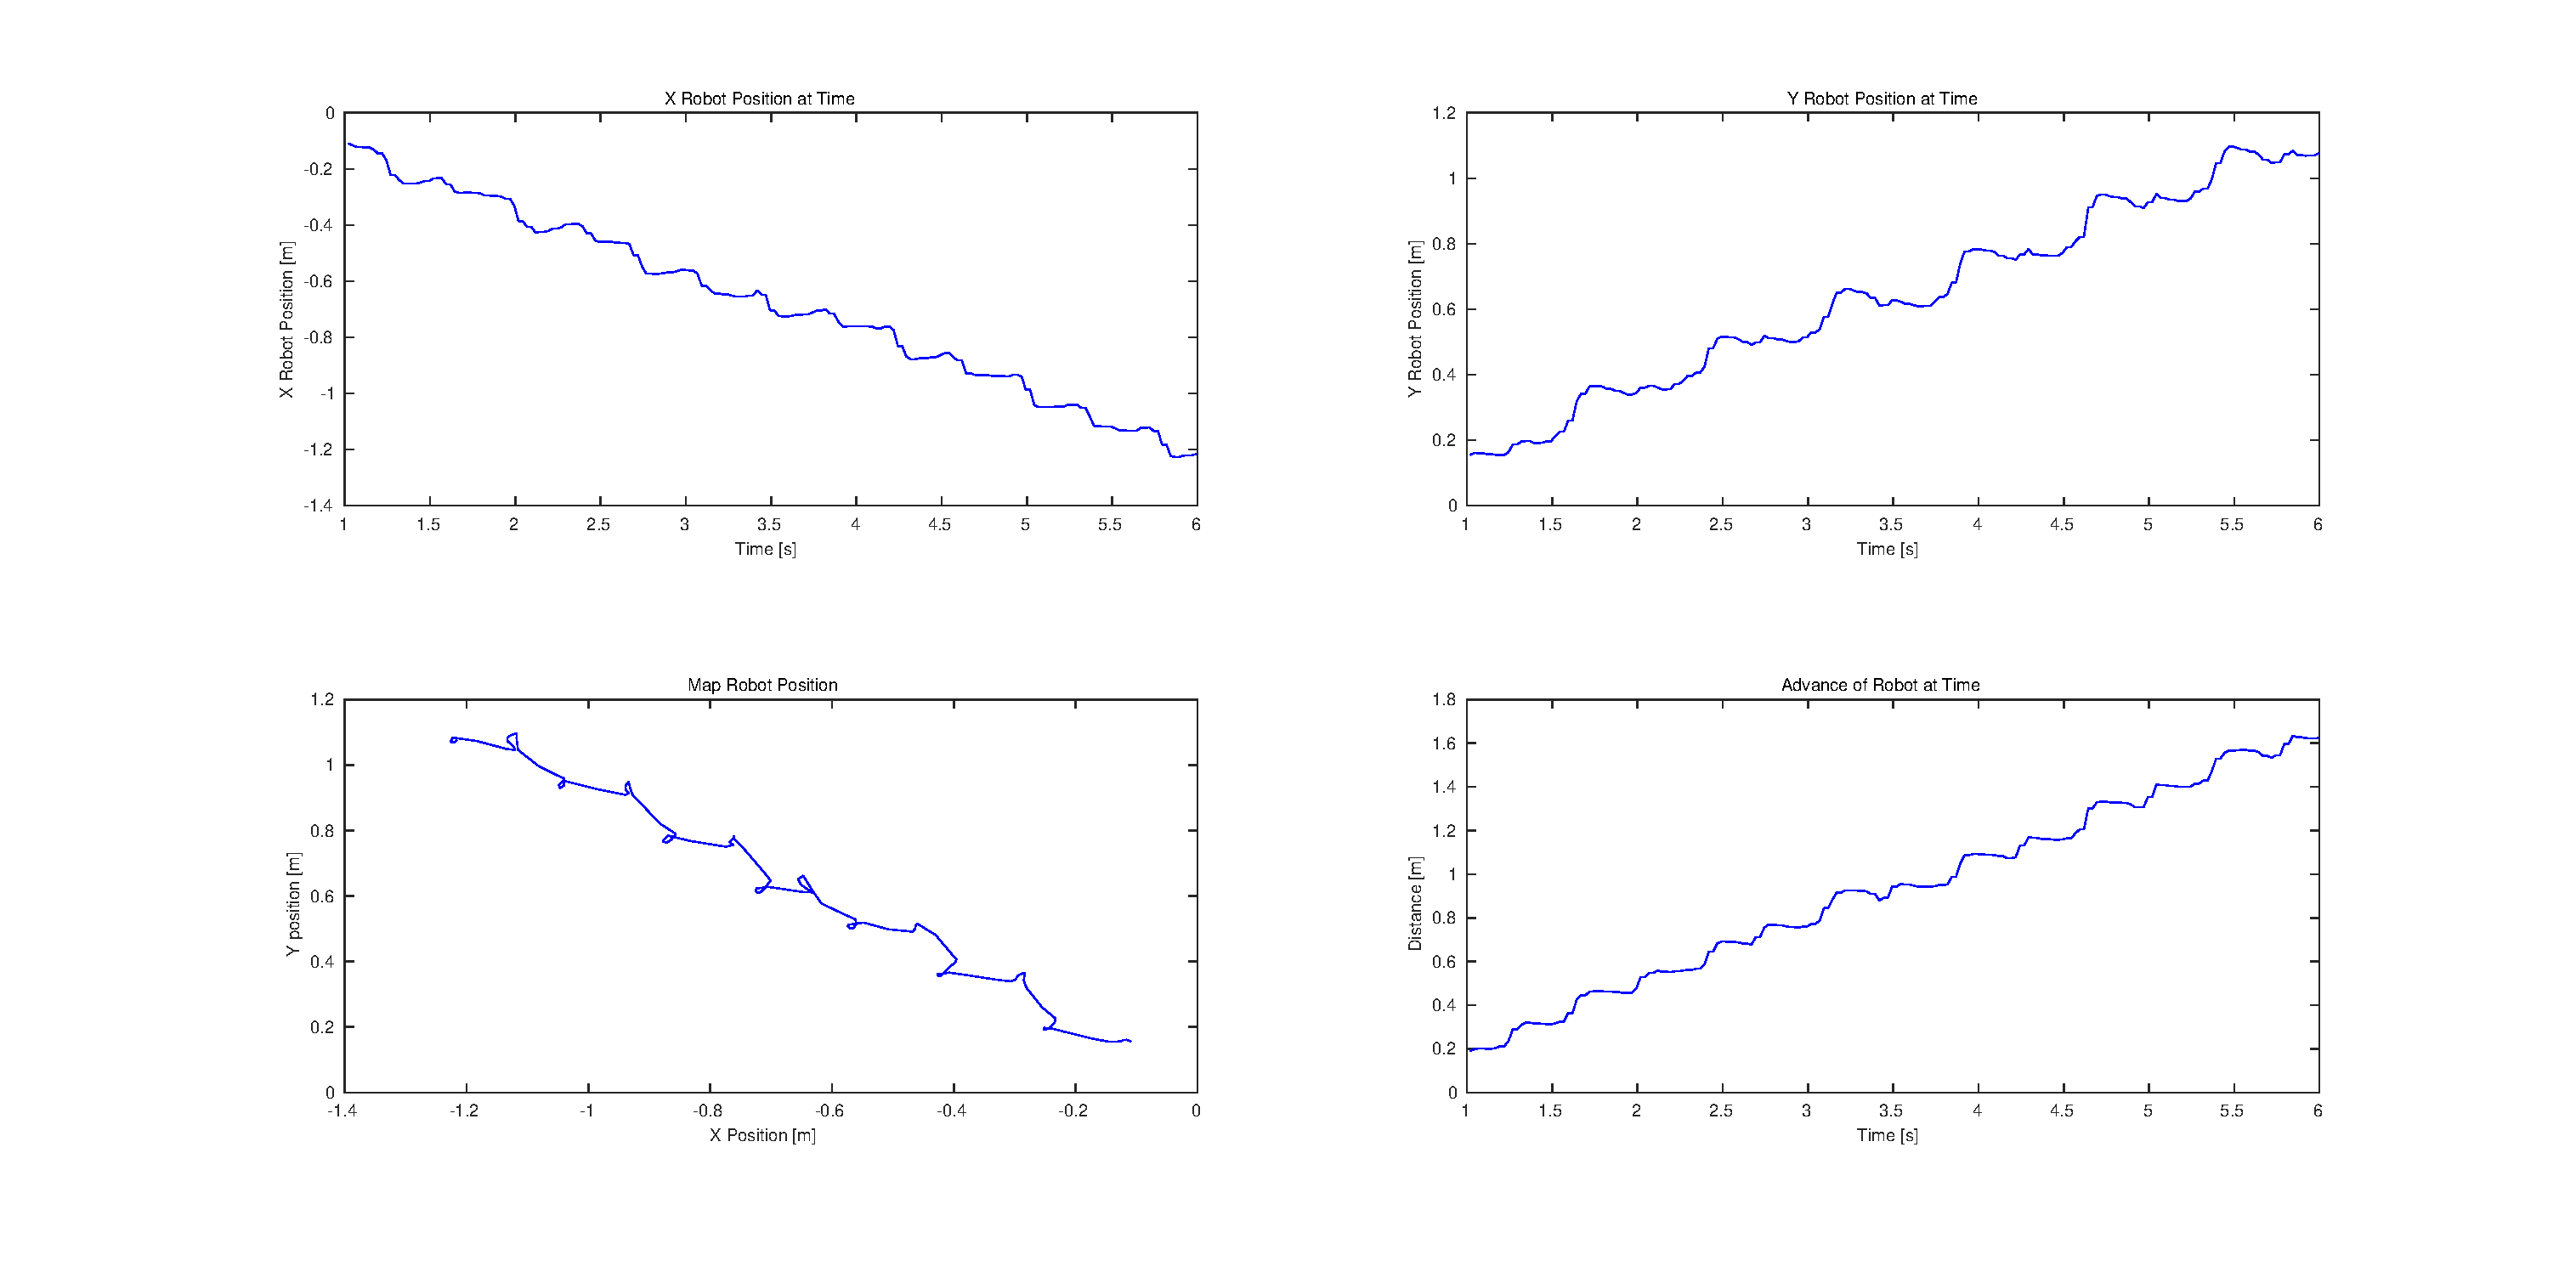
\includegraphics[width=\textwidth]{fig/ARGOV2_POSITION_HYPERNEAT.eps}
        \caption{HyperNEAT.}
        \label{fig:argov2_p_hyperneat}
    \end{subfigure}
    
    \begin{subfigure}[b]{\textwidth}
    	\centering
        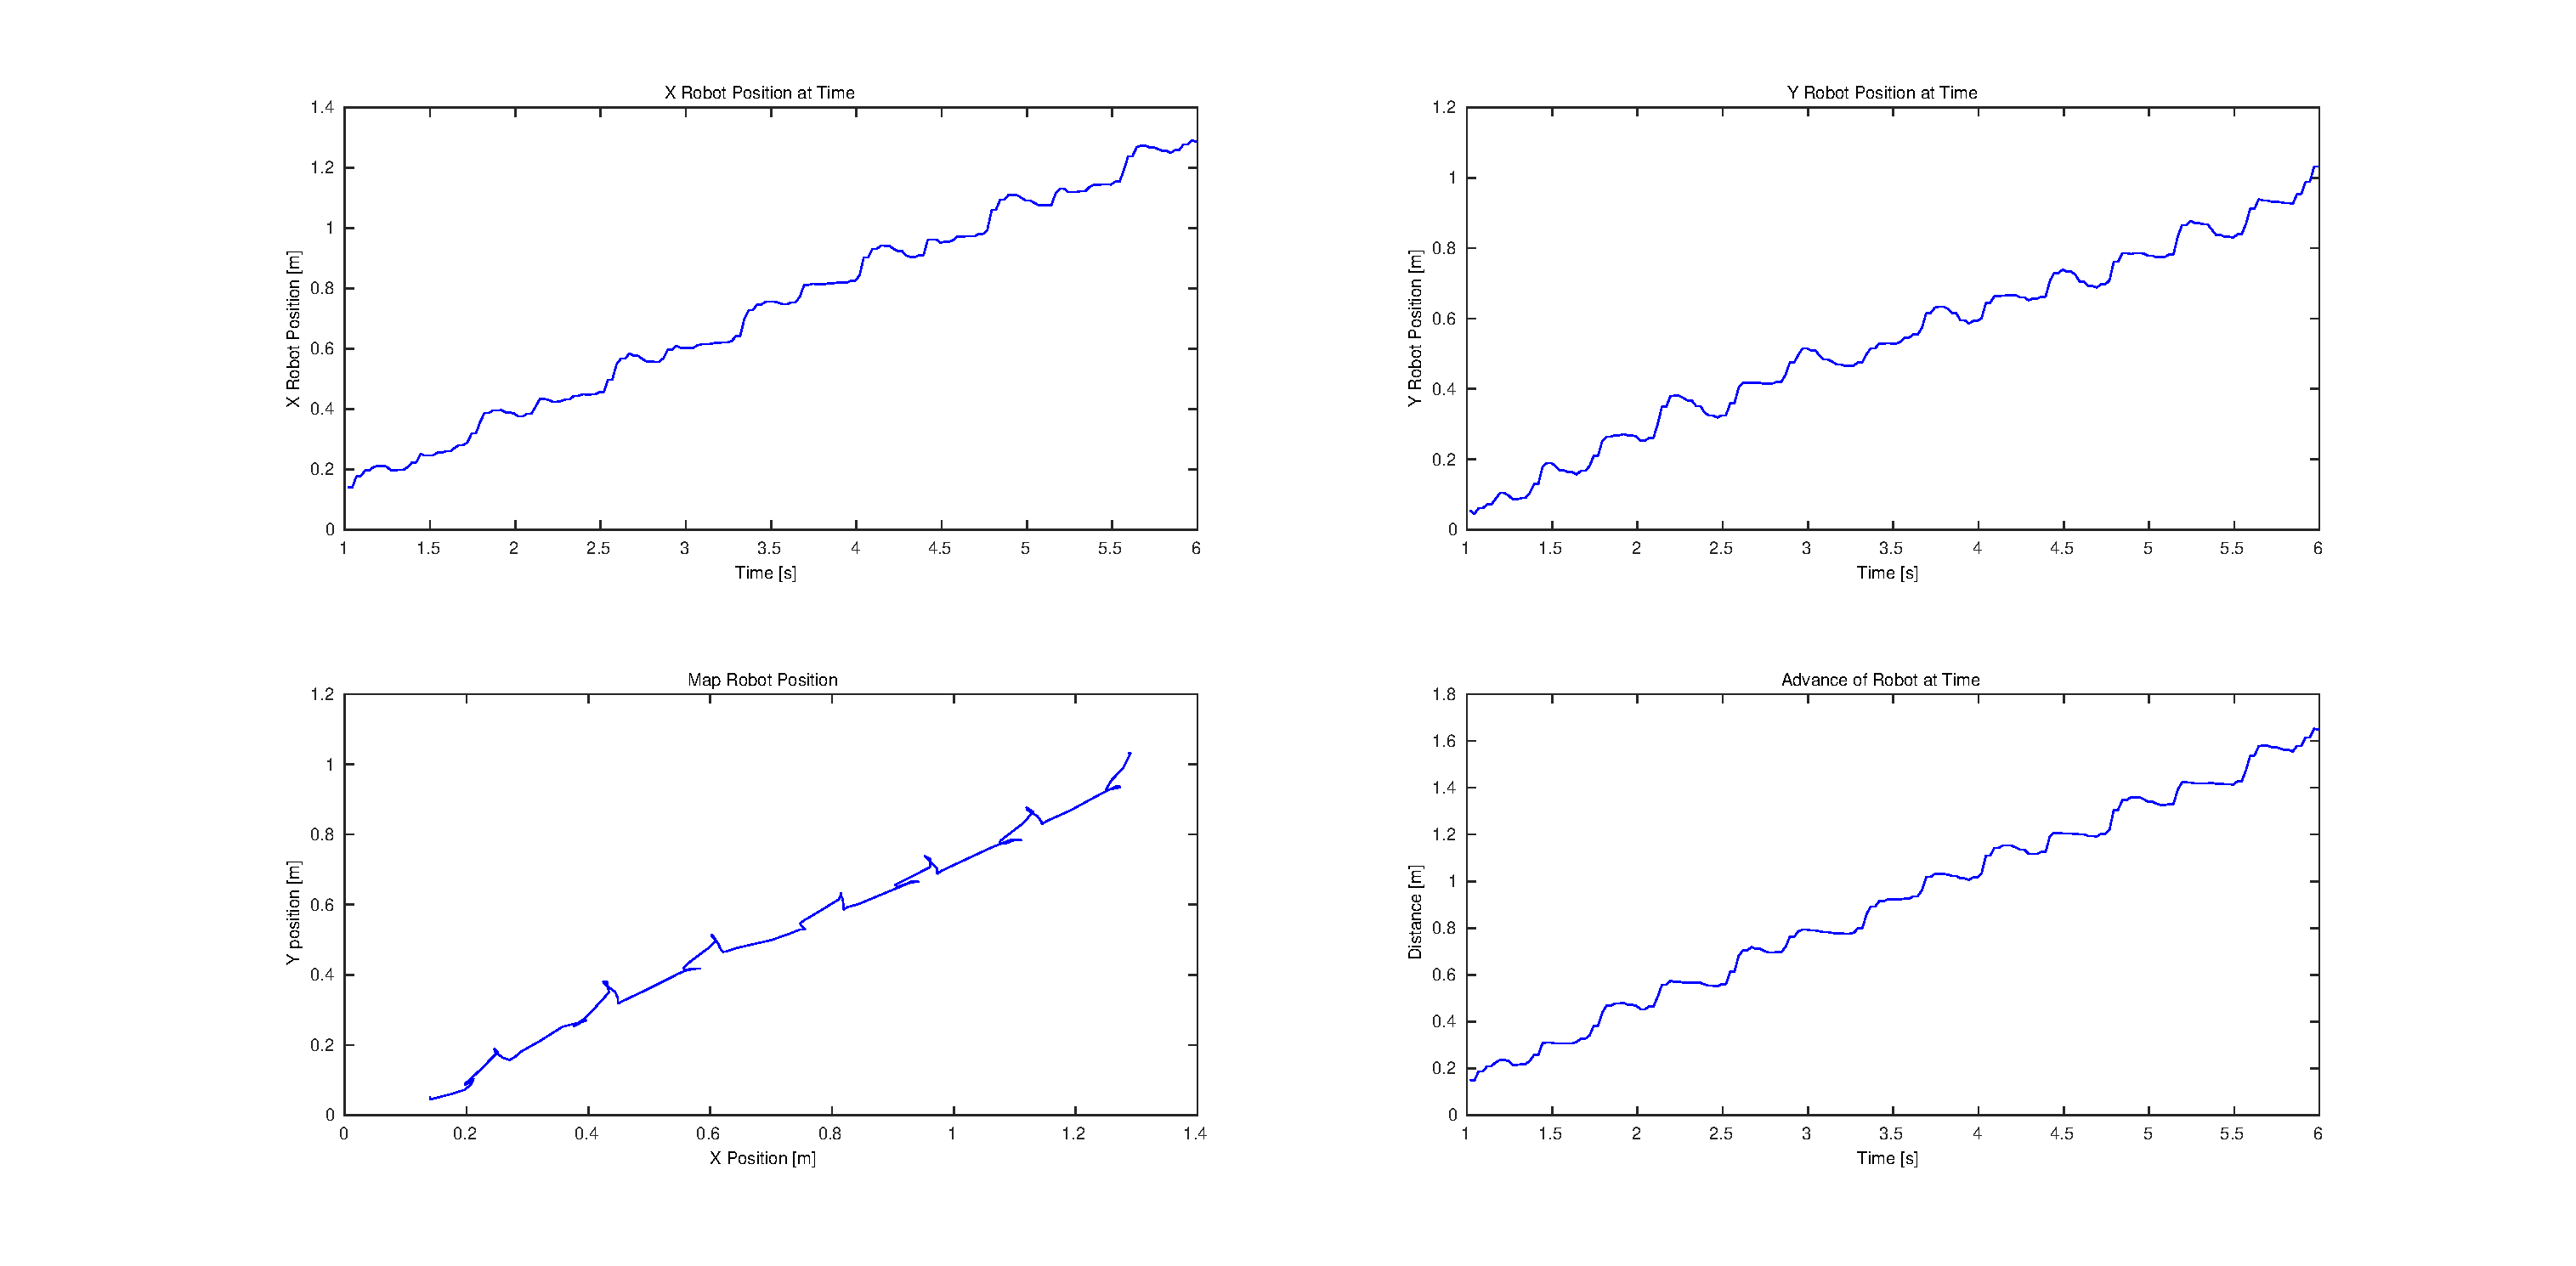
\includegraphics[width=\textwidth]{fig/ARGOV2_POSITION_TAUHYPERNEAT.eps}
        \caption{\(\tau\)-HyperNEAT.}
        \label{fig:argov2_p_tauhyperneat}
    \end{subfigure}
    \caption{\textbf{Desplazamiento de ArgoV2 en el escenario dado por HyperNEAT y \(\tau\)-HyperNEAT.} Los sets de gr�ficos presentes en esta figura muestran el desplazamiento de ArgoV2 a lo largo del escenario de simulaci�n en distintas medidas. Los gr�ficos superiores izquierdo y derecho muestra el desplazamiento en el tiempo del robot a lo largo del los ejes $x$ e $y$ respectivamente. EL gr�fico inferior izquierdo corresponde al desplazamiento del robot a lo largo del plano $xy$ del escenario. Finalmente el gr�fico inferior derecho corresponde a la distancia recta medida del robot hacia el punto de partida del escenario en el tiempo.}
    \label{fig:argov2_p}
\end{figure}

\clearpage
%
%%%%%%%%%%%%%%%%%%%%%%%%%%%%%%%%%%%%%%%%%%%%%%%%%%%%%%%%%%%%%%
%
\cleardoublepage
\chapter{Conclusiones y Trabajo futuro}
\label{cap:conclusiones}
\section{DISCUSION Y COMPARACION DE LOS RESULTADOS OBTENIDOS}

En este trabajo de memoria se ha implementado un nuevo m�todo de neuroevoluci�n, llamado \(\tau\)-HyperNEAT, con el objetivo de ponerlo a prueba en la tarde de generaci�n de caminatas en robots con extremidades m�viles. En particular, se ha planteado la hip�tesis de que este nuevo m�todo de neuroevoluci�n, al incorporar retardos de tiempo en las conexiones a lo largo de la red principal, tendr� mejoras en su desempe�o final y generar� caminatas con caracter�sticas cualitativas superiores.

Luego de analizar todos los resultados obtenidos a partir de los experimentos realizados es posible concluir lo siguiente.

\begin{enumerate}
\item En la tarea de generaci�n de caminatas, no hubo diferencias cuantitativas en los resultados obtenidos a trav�s de los m�todos HyperNEAT y \(\tau\)-HyperNEAT, obteni�ndose en ambos casos el mismo desempe�o de a cuerdo a las variables involucradas en el proceso de calificaci�n de las caminatas.
\item En la tarea de generaci�n de caminatas, \(\tau\)-HyperNEAT logr� desarrollar, casi en un 100\%, caminatas con movimientos arm�nicos y coordinados, similares a comportamientos vistos en la naturaleza. Esto pudo ser observado en los gr�ficos de las se�ales de los motores generadas por \(\tau\)-HyperNEAT, evidenciandose las diferencias y similitudes de fases vistas entre distintas extremidades y motores de una misma extremidad respectivamente.
\end{enumerate}

Ya que las capacidades de HyperNEAT para generar caminatas con movimientos arm�nicos y coordinados fueron pr�cticamente nulas frente a las capacidades mostradas por el m�todo \(\tau\)-HyperNEAT, es posible afirmar que este nuevo m�todo, al incorporar retardos de tiempo a lo largo de su red principal, logra afrontar y resolver de mejor manera problemas din�micos que involucran variables temporales, como lo es en particular, la generaci�n de caminatas en robots con extremidades m�viles.

\section{TRABAJO FUTURO}

Dados los resultados obtenidos en este trabajo de memoria, se considera que los siguientes
son temas para trabajo futuro, enfocados tanto en la generaci�n de caminatas como en la de cualquier tipo de experimento en donde se puedan aprovechar las capacidades de las redes HyperNEAT y \(\tau\)-HyperNEAT.

\begin{itemize}
\item Verificar las posibles variaciones en el desempe�o del m�todo \(\tau\)-HyperNEAT para distintos valores del retardo m�ximo ($\tau_{max}$) en las conexiones de la red.
\item Experimentar con diferentes configuraciones geom�tricas en el substrato de las redes HyperNEAT y \(\tau\)-HyperNEAT, con el objetivo de explotar al m�ximo las capacidades de ambas redes.
\item Formular y probar nuevas funciones de desempe�o para lograr clasificar de manera �ptima la correcta ejecuci�n de una caminata, favoreciendo siempre el proceso de evoluci�n de caminatas realmente efectivas y as� obtener mejores resultados.
\item Traspasar los resultados obtenidos en simulaciones a un entorno real, emulando de manera correcta las din�micas presentes en cada robot.
\end{itemize}
%
%------------------BIBLIOGRAF\'iA-----------------------------

%!TEX root = memoria.tex
\chapter{}

Introducci�n

\end{document}